% Input Macros (i.e. write your own macros file called MacroFile1.tex)
\include{Macros/MacroFile1}

\documentclass[oneside,12pt]{classes/CUEDthesisPSnPDF}

% CUSTOM PACKAGES
\usepackage{siunitx}
\usepackage{todonotes}
% \usepackage[superscript,biblabel]{cite}
\usepackage[super,comma,sort&compress]{natbib}

% for better equation alignment
\usepackage{IEEEtrantools}
% \usepackage{amsfonts}
% \usepackage{amssymb}
% \usepackage{amsmath}
\usepackage{pgfplots}
\usepgfplotslibrary{statistics}

% \ifpdf
%     \pdfinfo { /Title  (Goncalves NR - PhD Thesis)

% \ifpdf
%     \pdfinfo { /Title  (Goncalves NR - PhD Thesis)
%                /Creator (TeX)
%                /Producer (pdfTeX)
%                /Author (Nuno Reis Goncalves nrg30@cam.ac.uk)
%                /CreationDate (D:20150101000000)  %format D:YYYYMMDDhhmmss
%                /ModDate (D:20150101000000)
%                /Subject (Neural computation of depth from binocular disparity)
%                /Keywords (fMRI, vision, binocular disparity)}
%     \pdfcatalog { /PageMode (/UseOutlines)
%                   /OpenAction (fitbh)  }
% \fi

\title{Neural computation of depth from binocular disparity}

\ifpdf
  \author{\href{mailto:nrg30@cam.ac.uk}{Nuno Reis Gon\c{c}alves}}
  \collegeordept{\href{http://www.sid.cam.ac.uk}{Sidney Sussex College}}
  \university{\href{http://www.cam.ac.uk}{University of Cambridge}}
  \crest{\includegraphics[width=30mm]{UnivShield}} % insert the file name that contains the crest in-place of 'UnivShield'
\else
  \author{Nuno Reis Gon\c{c}alves}
  \collegeordept{Sidney Sussex College}
  \collegeordept{Department of Psychology}
  \university{University of Cambridge}
  \crest{\includegraphics[bb = 0 0 292 336, width=30mm]{UnivShield}}
\fi

%\renewcommand{\submittedtext}{change the default text here if needed}
\degree{Doctor of Philosophy}
\degreedate{January 2018}

% turn off those nasty overfull and underfull hboxes
\hbadness=10000
\hfuzz=50pt

% Put all the style files you want in the directory StyleFiles and usepackage like this:
\usepackage{style-files/watermark}

% other packages
\usepackage[font=footnotesize, labelfont={footnotesize,bf}]{caption}

% Comment out the next line to get single spacing
\onehalfspacing


\begin{document}

%\language{english}

% A page with the abstract on including title and author etc may be
% required to be handed in separately. If this is not so, then comment
% the below 3 lines (between '\begin{abstractseparte}' and 
% 'end{abstractseparate}'), normally like a declaration ... needs some more
% work, mind as environment abstracts creates a new page!
% \begin{abstractseparate}
%   \input{Abstract/abstract}
% \end{abstractseparate}

% Using the watermark package which is in StyleFiles/
% and to remove DRAFT COPY ONLY appearing on the top of all pages comment out below line
% \watermark{DRAFT COPY ONLY}

\maketitle

%set the number of sectioning levels that get number and appear in the contents
\setcounter{secnumdepth}{1}
\setcounter{tocdepth}{1}

\frontmatter % book mode only
\pagenumbering{roman}
% Thesis Dedictation ---------------------------------------------------

\begin{dedication} %this creates the heading for the dedication page

To Ksenia and Ivan

\end{dedication}

% ----------------------------------------------------------------------

%%% Local Variables: 
%%% mode: latex
%%% TeX-master: "../thesis"
%%% End: 

\include{acknowledgement/acknowledgement}
% Thesis Preface ------------------------------------------------

\begin{preface}      %this creates the heading for the preface

  My time as a graduate student at Cambridge was beyond intellectually stimulating. In the laboratory, I worked with a variety of experimental techniques, such as magnetic resonance imaging, spectroscopy and psychophysics. I had the wonderful opportunity of combining experiments with modeling. But most importantly, I had the privilege of working on the fascinating topic of stereopsis. Some of the most remarkable minds of the last two millenia --- Euclid, Da Vinci, Kepler, Newton, Descartes, and more --- have been at some stage bewildered by binocular vision and stereopsis. They were mostly struggling with the geometry of binocular vision (i.e. how the light is captured by the left and right eyes and how might that relate to depth in the environment). This is now well known. What we don't know yet is how the brain uses the signals captured by the left and right eyes to estimate depth. This is the central point of the thesis.
  
  Given that ultra-high field magnetic resonance imaging was not yet available in Cambridge, data acquisition for the experiments reported in Chapter 4 and 5 was performed in collaboration with the University of Nottingham and the University of Maastricht, respectively. The remaining contents of the thesis result from my own work, guided by my advisors Dr. Andrew Welchman and Prof. Zoe Kourtzi. I have not submitted any parts of the thesis for any other degree in the University of Cambridge or any other institution. The thesis does not exceed the word limit established by the Degree Committee for the Faculty of Biology.
  
\end{preface}

% ------------------------------------------------------------------------

%%% Local Variables: 
%%% mode: latex
%%% TeX-master: "../thesis"
%%% End: 

\include{abstract/abstract}

\tableofcontents
\listoffigures
% \listoftables
% \printnomenclature  %% Print the nomenclature
% \addcontentsline{toc}{chapter}{Nomenclature}

\mainmatter % book mode only
\include{introduction/introduction}
\chapter{`What not' detectors help the brain see in depth}
\ifpdf
    \graphicspath{{chapter1/chapter1-figs/PNG/}{chapter1/chapter1-figs/PDF/}{chapter1/chapter1-figs/}}
\else
    \graphicspath{{chapter1/chapter1-figs/EPS/}{chapter1/chapter1-figs/}}
\fi

\newcommand{\runningTitle}{`What not' detectors}
\markboth{\MakeUppercase{\thechapter. \runningTitle }}{\thechapter. \runningTitle}

% To do:
% [ ] check equations 
% [ ] replace citations
% [ ] include figures
% [ ] replace reference to main figures
% [ ] replace references to supplementary figures, etc...
% [ ] remove unnecessary italic and bold formatting 
% [ ] double check equations

This chapter reproduces the work associated with the following published manuscript: 

Goncalves NG \& Welchman AE. ``What not'' detectors help the brain see in depth. \textit{Current Biology}, 27, 1403--1412. 2017.

\section{Introduction}

Geometry dictates that a three-dimensional (3D) object viewed from the two eyes will (i) project features to different positions on the two retinae, and (ii) render certain portions visible to only one eye due to occlusion at the object's contours \cite{Wheatstone:1838xf}. Computational \cite{Julesz:1971uq,Marr:1976dq,Scharstein:2002by} and neurophysiological \cite{Cumming:2001jy} investigations over the past fifty years have focused almost exclusively on positional differences (i), as partial-occlusions (ii) are regarded as excessively under-constrained. Under this intuitive approach, by registering the positional difference of the same feature in the two eyes ({\it binocular disparity}), the brain could triangulate to infer the object's 3D structure. Thus, while the genesis of binocular information lies in image \emph {differences}, current understanding at the computational- and neural- levels stresses the centrality of identifying \emph {similarities} between the eyes to extract depth.

Within this framework, the fundamental challenge of stereopsis is described as solving the `correspondence problem' \cite{Julesz:1971uq,Marr:1976dq,Scharstein:2002by} whereby images of the same real-world feature are matched between the eyes. This is problematic because of `false matches' --- i.e., correspondences that conflate signals originating from different locations in 3D space. The principal means of identifying corresponding features is to consider a range of potential disparities and select the offset that maximises similarity between the eyes. This is captured computationally by the peak local cross-correlation. How might this be achieved by the brain? Current understanding is provided by the Disparity Energy Model of V1 neurons \cite{Ohzawa:1990cq, Fleet:1996tq, Qian:1997bu} in which binocular simple cells with disparity preference, $\delta_{pref}$, are combined by a complex cell preferring the same disparity (Fig. \ref{fig:c1f1}A). Using a population of cells with different $\delta_{pref}$, the brain could select the most active neuron to estimate depth.

However, from the perspective of finding correct matches, it is puzzling that many V1 neurons sense different things in the two eyes \cite{DeAngelis:1991mb, Prince:2002uq, Tsao:2003pi}. In particular, while binocular neurons can have receptive fields offset in location ({\it position disparity}), they often have different receptive field profiles in the two eyes ({\it phase disparity}) (Fig. \ref{fig:c1f1}B). The surprising implication is that phase neurons respond maximally to images that do not relate to a single physical feature in the world \cite{Read:2007nx}. What are such responses for? 

Here we suggest that V1 neurons should be understood as using a coding strategy designed to reduce uncertainty about the depth of the viewed scene. This involves the brain using both similar and dissimilar image features to infer depth. We show that long-standing puzzles in binocular vision at the physiological- and perceptual- levels can be understood by mixing feature detection with \emph {proscription}. Specifically, by sensing \emph {dissimilar} features the brain gains valuable information that drives suppression of unlikely interpretations of the scene. Our approach explains challenges to the standard treatment of disparity (i), and importantly, also accounts for (ii) partial occlusions that have long evaded explanation because of their incompatibility with registering depth based on peak cross-correlation. 

\section{Results}

We start by considering known properties of binocular neurons from a statistical perspective \cite{Shannon1948}, to demonstrate that properties that have long seemed puzzling in fact suggest optimal coding. Position-disparity units (Fig. \ref{fig:c1f1}B, purple) are easily understood from the traditional perspective: a viewed object will project its features to different locations on the two retinae, so a binocular unit could simply offset the receptive field location for the two eyes. Phase-disparity units (Fig. \ref{fig:c1f1}B, orange), by contrast, have a different receptive field structure in the two eyes. This means they respond best to stimulation that could not originate from a single physical feature in the world. We contrasted phase- and position- encoding by computing Shannon information \cite{Shannon1948} as a function of stimulus disparity (see Methods), where simple units were modeled as linear filters followed by a rectified squaring non-linearity \cite{Ohzawa:1990cq}. Because of the larger change in firing of the phase units, they provide more information about the viewed stimulus than position units (Fig. \ref{fig:c1f1}C). Importantly, the peak information provided by a phase unit is not at the traditionally-labelled $\delta_{pref}$ (i.e., peak firing rate), meaning that the Disparity Energy Model's architecture (Fig. \ref{fig:c1f1}A) of collating signals from units with the same $\delta_{pref}$ is likely to be suboptimal. We then examined encoding in a small population of simple units with \emph {position}, \emph {phase} or \emph {hybrid} receptive fields. We found that \emph {hybrid} encoding (i.e. combined phase and position shifts: {Fig. \ref{fig:c1f1}B) conveys more information than either pure phase or position encoding (Fig. \ref{fig:c1f1}D). This suggests that the abundance of hybrid selectivity in V1 neurons \cite{DeAngelis:1991mb, Prince:2002uq, Tsao:2003pi} may relate to optimal encoding. 

\begin{figure}[!h]
  \centering
  \includegraphics{chapter1/chapter1-figs/Fig1.pdf}
  \caption[Disparity encoding and Shannon information.]{Disparity encoding and Shannon information. ({\bf A}) The canonical Disparity Energy Model. Simple and complex units have the same preferred disparity, $\delta_{pref}$. ({\bf B}) Simple cells encode disparity using differences in receptive field: position ({\it position} disparity), structure ({\it phase} disparity), or both ({\it hybrid}). ({\bf C}) Mean response of model simple units to 100,000 stereograms (top) and the corresponding Shannon information (bottom). Pink {\it vs}. yellow series contrast pure position vs. phase ($\pi/2$) encoding, both with $\delta_{pref}$=4. Considering units between pure position and pure phase encoding produces a graceful morphing in the shapes of the curves. ({\bf D}) Shannon information for a small population ($N=5$) of simple units with position, phase or hybrid sensors. (Computing Shannon information for larger populations was computationally prohibitive). Error bars show SD over 1000 populations with randomly distributed phase and/or position shifts. Horizontal lines depict the upper limit on information determined by a population with uniformly spaced units.}
  \label{fig:c1f1}
\end{figure}


To test the idea that V1 neurons are optimised to extract binocular information, we developed a model system shaped by exposure to natural images. We implemented a binocular neural network (BNN, Fig. \ref{fig:c1f2}A) consisting of a bank of linear filters followed by a rectifying non-linearity. These `simple units' were then pooled and read out by an output layer (`complex units'). The binocular receptive fields and readout weights were optimised by supervised training on a near {\it vs}. far depth discrimination task using patches from natural images (Supplementary Figure \ref{fig:c1fs1}). Thereafter, the BNN classified depth in novel images with high accuracy ({\it A}=99.23\%). 

\begin{figure}[!h]
  \centering
  \includegraphics{chapter1/chapter1-figs/Fig2.pdf}
  \caption[The Binocular Neural Network.]{The Binocular Neural Network (BNN). ({\bf A}) Network architecture: left and right images are filtered by simple units (28 binocular convolutional kernels), linearly rectified, and then readout by two output units. The form of the (i) receptive fields and (ii) readout weights was determined through back-propagation optimisation on {\it near vs. far} depth discrimination using patches from stereoscopic natural images \cite{Li:2014ik}. The network learnt 21,254 parameters through exposure to 32,300 image pairs. ({\bf B}) The BNN's optimised receptive fields resembled Gabor functions (mean explained variance by fitting Gabors to the 28 binocular receptive fields was $R^2=0.95$, $s.d.=0.049$) and V1 receptive fields \cite{DeAngelis:1991mb} ({\bf C}) Summary of position and phase encoding by the simple units; representative units from (B) highlighted using colour. Note very few units show pure position or phase offsets. See also Supplementary Figure \ref{fig:c1fs1} and Supplementary Figure \ref{fig:c1fs2}.}
  \label{fig:c1f2}
\end{figure}


\subsection{Optimisation with natural images produces units that resemble neurons}

The optimised structure of the BNN resembled known properties of simple and complex neurons in three main respects. First, simple units' receptive fields were approximated by Gabor functions (Fig. \ref{fig:c1f2}B) that exploit hybrid encoding (Fig. \ref{fig:c1f2}C; Supplementary Figure \ref{fig:c1fs2}) \cite{DeAngelis:1991mb, Prince:2002uq, Tsao:2003pi} with physiologically-plausible spatial frequency bandwidths (mean=2.3 octaves). Second, like V1 neurons, the BNN supported excellent decoding of depth in correlated random dot stereogram (cRDS) stimuli (Fig. \ref{fig:c1f3}A) ({\it A}=99.93\%; {\it CI}\textsubscript{95\%}=99.87\%, 99.98\%) that are traditionally used in the laboratory, despite being trained exclusively on natural images. Third, we tested the BNN with anticorrelated stimuli (aRDS) where disparity is depicted such that a dark dot in one eye corresponds to a bright dot in the other (Fig. \ref{fig:c1f3}A). Like V1 complex cells \cite{Ohzawa:1990cq,Cumming:1997ve, Samonds:2013cs}, disparity tuning was inverted and attenuated (Fig. \ref{fig:c1f3}B), causing systematic mispredictions of the stimulus depth ({\it A}=8.83\%; {\it CI}\textsubscript{95\%}=7.62\%, 9.03\%). 

\begin{figure}[!h]
  \centering
  \includegraphics[width=14cm,keepaspectratio]{chapter1/chapter1-figs/Fig3.pdf}
  \caption[ BNN response to correlated and anticorrelated random-dot stereograms.]{ BNN response to correlated and anticorrelated random-dot stereograms. ({\bf A}) Cartoons of correlated (cRDS, green) and anticorrelated (aRDS, pink) dot patterns with red-green anaglyph demonstrations. ({\bf B}) Complex unit's disparity tuning curve for cRDS {\it vs}. aRDS; shaded area shows $CI_{95\%}$. ({\bf C}) Distribution of amplitude ratios for cRDS {\it vs}. aRDS for the BNN (grey histogram; 5000 resamples), and macaque V1 neurons. Amplitude ratios were determined based on Gabor fits (average explained variance, $R^2=0.945$) ({\bf D}) Representation of the weighted readout of the simple units. Units are ordered by their readout weight with {\it far}- preferred units at the top. ({\bf E}) Mean activity for simple units in response to cRDS and aRDS. ({\bf F}) Summary of excitatory (red) and suppressive (blue) drive to the output units for cRDS {\it vs.} aRDS. This represents the sum of the weighted simple unit activity split into the excitatory (positive weights) and suppressive (negative weights) components. Error bars (hardly visible) show $CI_{95\%}$. See also Supplementary Figure \ref{fig:c1fs3}.}
  \label{fig:c1f3}
\end{figure}


V1 complex cell attenuation for aRDS is not explained by the canonical energy model, necessitating extensions that have posited additional non-linear stages \cite{Lippert:2001ur, Haefner:2008jg, Samonds:2013cs, Read:2002kx}. However, the BNN naturally exhibited attenuation: by computing the ratio of responses to aRDS {\it vs}. cRDS, we found striking parallels to V1 neurons \cite{Cumming:1997ve, Samonds:2013cs} (Fig. \ref{fig:c1f3}C). There was a divergence between the two comparison physiological datasets for low amplitude ratios, with our model closer to Samonds et al \cite{Samonds:2013cs}. We speculate that this relates to the disparity selectivity of the sampled neurons: Cumming and Parker \cite{Cumming:1997ve} recorded closer to the fovea where sharper disparity tuning functions might be expected. Accordingly, we observed greater attenuation (i.e., lower amplitude ratios) when the BNN was trained on multiway classifications (e.g., 7 output units, rather than 2) which produced more sharply tuned disparity responses (Supplementary Figure \ref{fig:c1fs3}). Together, these results show that inversion and attenuation for anticorrelation appear in a system optimised to process depth in natural images. 


The traditional account of aRDS is that they simulate `false matches' that the brain discards to solve the correspondence problem \cite{Tanabe:2004mw,Janssen:2003fk}. An alternative possibility, however, is that aRDS responses reflect a computational mechanism for extracting depth. To test this idea, we interrogated the BNN by ordering simple units by their readout weights (Fig. \ref{fig:c1f3}D) and then visualising the activity evoked by different stimulus types (Fig. \ref{fig:c1f3}E). The weighted-readout of simple unit activity defines the overall excitatory and suppressive drive to complex units in the network. We found that presenting aRDS led to a striking increase in the activity of the non-preferred simple units, while the activity of the preferred units was more-or-less unchanged. The consequence of this is that when this activity is readout it causes increased suppression at the preferred disparity (Fig. \ref{fig:c1f3}F). This changed the net drive to the complex unit from excitation to suppression (inversion), while the comparatively smaller difference between the excitatory and suppressive drives for aRDS produced a reduced amplitude (attenuation). Thus, attenuation and inversion can be understood based on changing the balance of excitation and suppression, without necessitating additional processing stages. 


To ensure that these parallels between the BNN and neurophysiology were not incidental, we tested whether he BNN produces outputs that are well-matched to the input stimuli. We used an optimisation procedure that started with random noise input images and iteratively adjusted the images such that the activity of a given complex unit was maximized (Fig. \ref{fig:c1f4}A). Following optimisation, the stimuli that best activated the complex units resembled a contrast edge horizontally translated between the eyes (Fig. \ref{fig:c1f4}B). Thus, the BNN is optimised for the translation of visual features that results from binocular viewing geometry \cite{Wheatstone:1838xf}. Importantly, this is achieved using simple units that respond predominantly to different features in the two eyes (Fig. \ref{fig:c1f2}B), which are traditionally understood as `false' matches (i.e., that do not correspond to the same physical real-world object). In other words, the BNN extracts depth structure without explicitly `solving the correspondence problem'. 

\begin{figure}[!h]
  \centering
  \includegraphics{chapter1/chapter1-figs/Fig4.pdf}
  \caption[Optimal stimuli for the binocular neural network.]{({\bf A}) Computing the optimal stimulus for a complex unit. Starting with random noise inputs, the algorithm computed the gradient of complex unit activity with respect to the input images. It iteratively adjusted the inputs to maximize the complex unit's activity. ({\bf B}) Snapshots of three iterations during optimisation: a consistent On-Off pattern emerges in the left and right eyes, horizontally translated to match the preferred disparity of the unit. ({\bf C}) This pattern remains when `lesioning' the BNN of 25\% of the simple units that use position encoding. ({\bf D}) Removing highly-weighted hybrid units leads to input images that are unrealistic.}
  \label{fig:c1f4}
\end{figure}


To strengthen this conclusion, we examined the consequences of `lesioning' the BNN by removing 25\% of its units. In particular, we removed units with near-zero phase disparities (i.e., the seven units within $\pm \frac{\pi}{4}$ of zero phase offset) that are therefore best described as position disparity units that sense similar features in the two eyes. First, we considered decoding performance and found no effect on accuracy ({\it A\textsubscript{Pos}}=99.97\%, {\it CI}\textsubscript{95\%}=99.92\%,100\%; {\it p}=.76; Supplementary Figure \ref{fig:c1fs2}D). To situate this null result in the context of arbitrarily removing a quarter of the units, we also computed decoding performance when we randomly removed seven simple units. In this case, decoding performance dropped considerably (Supplementary Figure \ref{fig:c1fs2}D), and there was only 3.8\% chance of obtaining a value greater than {\it A\textsubscript{Pos}}. This suggests that the pure position units contribute little to registering the binocular information by the BNN: they are given little weight so removing them has little effect relative to removing phase or hybrid units. Second, we computed the optimal stimulus for the lesioned BNN (Fig. \ref{fig:c1f4}C), finding little change relative to the uncompromised network. This null result was not inevitable: removing other simple units resulted in unrealistic images (Fig. \ref{fig:c1f4}D). Together, this indicates that the BNN does not critically depend on binocularly-matched features.

But how does the BNN extract depth using mismatches, and why should it respond to anticorrelated features? Under the traditional approach, this is a puzzle: a physical object at a given depth would not elicit a bright feature in one eye and a dark feature in the other. However, as we have seen, anticorrelation at the preferred disparity of a complex cell leads to strong suppression. This suggests a role for \emph {proscription}: by sensing \emph {dissimilar} features the brain extracts valuable information about unlikely interpretations.

\subsubsection*{\textit{The BNN accounts for unexplained perceptual results}}

 If proscription has a perceptual correlate, then stereopsis should be affected by the availability of dissimilar features in the scene, an idea we now explore. First, seeing depth should be easier when there is more potential for anticorrelation at the \emph {incorrect} disparity. This logic naturally explains a long-standing puzzle from the psychophysical literature \cite{Harris:1995va, Read:2011im} that demonstrated better judgments for stimuli comprising dark and bright dots (mixed polarity) compared to only dark or only bright dots (single polarity) (Fig. \ref{fig:c1f5}A). This result is difficult to accommodate within the Disparity Energy Model because correlation is largely unaffected by differences in the mean or amplitude of the input signals \cite{Read:2011im}.

\begin{figure}[!h]
  \centering
  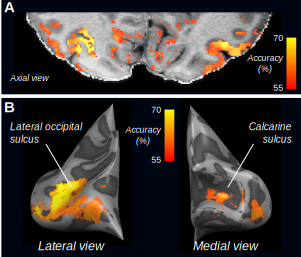
\includegraphics{chapter1/chapter1-figs/Fig5.pdf}
  \caption[The BNN mirrors properties of human stereopsis.]{ The BNN mirrors properties of human stereopsis. ({\bf A}) Mixed vs. single polarity stereograms. Single polarity stereograms were either all dark, or all bright. The task was to discriminate the step arrangement of the stereogram. Anaglyphs designed for red filter over right eye. ({\bf B}) Proportion of correct choices of the model after 1000 trials. ({\bf C}) Efficiency ratio for mixed {\it vs}. single stimuli measured psychophysically \cite{Harris:1995va} and for the BNN. (Note: the BNN was optimised on natural images, {\it not} random dot stereograms) ({\bf D}) Difference between mixed and single stimuli in terms of the excitatory {\it vs}. suppressive drive to the non-preferred output unit. Error bars $CI_{95\%}$. See also Supplementary Figure \ref{fig:c1fs4}.}
  \label{fig:c1f5}
\end{figure}

 We assessed the BNN's performance on mixed {\it vs}. single polarity stereograms (Fig. \ref{fig:c1f5}B), finding a benefit for mixed stimuli that was very closely matched to published psychophysical data \cite{Harris:1995va, Read:2011im} (Fig. \ref{fig:c1f5}C). What causes this improvement? As reviewed above, the network depends on the activity of the simple units moderated by readout weights. Presenting mixed {\it vs}. single polarity stimuli increases the simple unit activity, in turn changing the excitatory and suppressive drives to complex units. We found that mixed stimuli produce greater excitation for the preferred output unit and increased suppression to the non-preferred unit (Fig. \ref{fig:c1f5}D). 

We carried out a number of controls to ensure that the BNN's performance was not artefactual. In particular, contrasting mixed {\it vs}. single polarity stereograms is complicated by low-level stimulus changes (e.g., overall luminance, or stimulus intensity range) that could act as covariates which underlie performance \cite{Read:2011im}. We directly manipulated covariate properties (Supplementary Figure \ref{fig:c1fs4}), finding that the benefit for mixed stimuli persisted in all cases. We also tested the specificity of this result to the BNN's non-linearity \cite{Read:2011im}. Changing the nonlinearity to an unrectified squaring operation did not change the result (Supplementary Figure \ref{fig:c1fs4}). These controls indicate that the improvement for mixed stimuli generalises over perturbations of the stimuli and network architecture. These results suggest that performance improves for the mixed stimuli because of the opportunity to gain stronger evidence for the true disparity in conjunction with using mismatched features (i.e., dark-to-bright correspondences) as evidence against the incorrect disparity (i.e., proscription). This could be implemented {\it in vivo} using suppressive inputs to V1 neurons \cite{Tanabe:2011pt}.

A second line of evidence in favour of proscription comes from considering situations regarded as too difficult for accounts of stereopsis based on peak correlation. Under natural viewing, certain features are visible to one eye but not the other (Fig. \ref{fig:c1f6}A). The brain exploits such unpaired elements, `Da Vinci' stereopsis, to support depth perception \cite{Gillam:1988lo, Nakayama:1990fc}. However, these stimuli pose a severe challenge to traditional stereo-algorithms because there are no matching features \cite{Anderson:1994tp}. We tested the BNN on a stimulus with unpaired features around a zero-disparity target (Fig. \ref{fig:c1f6}B). Because the target was not displaced in depth, there are no binocular corresponding features to compute the depth relationship. However, the BNN predicted the ordinal depth structure experienced by observers for the edge regions (Fig. \ref{fig:c1f6}B), and this result generalised to stimuli with different luminance configurations (Supplementary Figure \ref{fig:c1fs5}). The BNN thus extracts critical signals that may provide the foundation for a full perceptual interpretation when used in conjunction with processes such as figure-ground segmentation at further stages of visual processing \cite{Ban:2015cr, Tsirlin2014}.

\begin{figure}[!h]
  \centering
  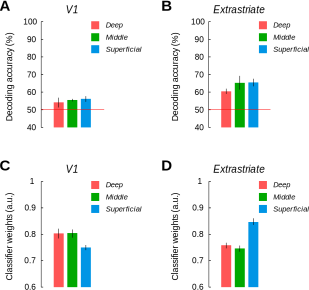
\includegraphics{chapter1/chapter1-figs/Fig6.pdf}
  \caption[Ordinal depth prediction with ill-defined or ambiguous disparities.]{Ordinal depth prediction with ill-defined or ambiguous disparities. ({\bf A}) Illustration of occlusion around the edges of objects. ({\bf B}) `Da Vinci' stereopsis. {\it Left}: Illustration of half-occlusions (black flanks) produced by viewing geometry; {\it Centre}: `Da Vinci' stereograms for cross-eyed fusion; {\it Right}: depth map from the BNN. ({\bf C}) Wallpaper illusion. {\it Top}: Ambiguous pattern. The vertical stripes can be matched by a nasal or temporal shift, making both {\it near} and {\it far} global matches valid. Cross-eyed fusion allows the reader to experience alternation. The BNN does not detect a clear depth. {\it Bottom}: Biasing perception by changing background luminance leads to a concomitant shift in the BNN's interpretation. ({\bf D}) The net drive between excitation and suppression that underlies the shift in prediction, contrasting the ambiguous case and disambiguated cases. Note: for all these examples it is clear that the BNN has not `reproduced' the percept: rather the network provides key signals that may provide the foundations for typical percepts. See also Supplementary Figure \ref{fig:c1fs5}. }
  \label{fig:c1f6}
\end{figure}

Finally, we tested the BNN on the classic `wallpaper illusion' \cite{Brewster:1844jy}, in which periodic patterns yield ambiguous depth percepts. When disparity matches were ambiguous, the disparity-sign map did not identify a clear depth edge (Fig. \ref{fig:c1f6}C). However, by manipulating the background luminance to bias matching \cite{Anderson:1994fk}, we found that the BNN predicted the perceptual interpretation of the stereograms in the edge regions. This was achieved by changing the net excitatory-suppressive drive at the half-occluded regions, where disambiguation occurs (Fig. \ref{fig:c1f6}D). This is compatible with early processing of half-occluded edge regions in V1, providing an initial basis for subsequent depth interpolation supported by extrastriate cortex \cite{Mckee:2007da} or via recurrent connectivity within V1.

Together, these results indicate that, without being trained on such displays, the BNN's combination of detection and proscription provides a natural foundation for typical percepts. The simple units of the BNN exploit receptive fields that capture a continuum of similarities and differences between the binocular images, contrasting with the standard approach to binocular vision that emphasised the importance of correct matches. While individual units in the BNN are not specialised to identify the same feature in the two images, the aggregate readout activity classifies depth with high accuracy and complex units respond best to physically-realistic displacements of a single object.

\subsubsection*{Detection and proscription combine to facilitate sensory estimation}

We have seen that the BNN generalises well from its training set and accounts for both neurophysiological and perceptual phenomena. However, the network's multiple parameters may act as a barrier to a detailed understanding of its operation. We therefore sought to explain the BNN's behaviour in theoretical terms by deriving a low-parameter closed-form model that captures its key characteristics. Our starting point was to observe that a low-dimensional rule relates the BNN's simple units and their readout: weights are proportional to the cross-correlogram between the (left and right) receptive fields ({\it R}=0.89; {\it p}$<$.001) (Supplementary Figure \ref{fig:c1fs6}}). 


The key intuition behind this relationship is that receptive fields capturing a positive correlation at disparity $\delta_{i}$ (i.e. the lag of the cross-correlogram) should be read out by a complex unit with preferred disparity $\delta_{i}$ using a positive (i.e. excitatory) weight. Conversely, if the simple unit captures a negative correlation at disparity $\delta_{i}$, the complex unit should read out its activity using a negative (suppressive) weight. In other words, the same simple units can be read out with detection or proscription to provide a population-based estimate of the depth of the viewed scene.


We show formally (Methods) that using weights determined by the cross-correlogram of the left and right receptive fields is optimal under reasonable assumptions, and propose a Binocular Likelihood Model captured by a simple equation,
\[
\log L(\delta) = \sum_{i=1}^N r_i (W_L \star W_R)_i [\delta].
\]
This relationship states that the activity of a complex unit that prefers a given disparity $\delta$ (expressed as a log likelihood, $L(\delta)$), is given by a weighted sum of simple unit activity, $r_i$. The weights correspond to the cross-correlation, $(W_L \star W_R)_i$, between the left and right receptive fields of simple unit $i$ at disparity $\delta$ (Fig. \ref{fig:c1f7}). To demonstrate the model, we implemented an instantiation that produces disparity tuning curves for correlated and anticorrelated RDS that closely resemble V1 complex cells (Supplementary Figure \ref{fig:c1fs7}). This instantiation included a single spatial frequency channel, so the model does not require pooling across spatial scales to exhibit attenuation for aRDS. The model's key parameters are simply the receptive fields of the input units. This suggests that a fixed, stimulus-independent architecture explains key binocular phenomena, possibly without supervised learning.  


\begin{figure}[!h]
  \centering
  \includegraphics{chapter1/chapter1-figs/Fig7.pdf}
  \caption[Binocular Likelihood Model.]{Binocular Likelihood Model. Input images are processed by a population of simple units that perform linear filtering followed by nonlinear rectification. The activity of a given simple unit ($r_i$) is readout by multiple complex units. A simple unit's readout weights vary over complex units, where the readout weight is defined by the cross-correlation of the simple unit's left and right receptive fields. The activity of the population of complex cells encodes the likelihood function for stimulus disparity. See also Supplementary Figure \ref{fig:c1fs6} and Supplementary Figure \ref{fig:c1fs7}.}
  \label{fig:c1f7}
\end{figure}


\section{Discussion}

Traditional understanding of stereopsis at the computational-, neural- and perceptual- levels has focused on the idea that peak correlation should be used to identify similar features and discard false matches. The logic underlying this approach is based on inverting the geometry that maps objects at different locations in space onto different portions of the two retinae. However, here we show that envisaging neurons as units that match up the features of objects in the world fails to account for known properties of neurons, and overemphasises the role of similarity in a system whose fundamental benefit lies in differences between the images sensed by the two eyes. 

We demonstrate that V1 neurons have properties ideally suited to extract binocular information, rather than simply searching for matching features. We formalise a Binocular Likelihood Model that provides a unifying account for previously puzzling properties of V1 neurons as well as perceptual phenomena that challenge the standard approach. This model highlights the interplay between feature detection and proscription for perceptual inference. This mix of evidence for and against likely interpretations may represent a general strategy for perceptual integration both within and between sensory modalities.

\subsubsection*{Understanding the functional role of sensory neurons}

Understanding the coding strategies of sensory neurons represents a longstanding challenge. A historically pervasive idea is that sensory neurons act as `feature detectors', signalling evidence for the occurrence of a particular feature in the environment \cite{Barlow:1953ep, Lettvin:1959gs}. For instance, orientation-selective neurons could indicate the presence of a particular tilted edge in a visual display \cite{HUBEL:1959tz}. It has long been recognised that natural images shape this selectivity \cite{Barlow:1961fe, Simoncelli:2001dn}, with neural responses optimised for efficient representation of the statistical regularities of the environment \cite{Karklin:2009hl, Li:1994jm}. 

Here we take the approach of quantifying the information conveyed by early sensory neurons that are sensitive to binocular disparity using information analysis, and then by implementing a neural network optimised by exposure to natural images. This provides insight into the functional purposes of disparity representations at the neural and perceptual levels. Our findings on the utility of hybrid receptive fields for disparity encoding are consistent with work that used dimensionality reduction to estimate the optimal disparity filters \cite{Burge:2014qj}. In particular, our observation that hybrid units capture greater Shannon information is consistent with the idea that hybrid encoding maximises disparity estimation accuracy. Moreover, hybrid receptive fields are suggested to minimise the statistical redundancy of binocular responses \cite{Okajima:2004cy,Hunter:2015kx, Hunter:2016gb}, suggesting an additional factor driving the brain's use of hybrid units.

\subsubsection*{Understanding the encoding properties of the BNN}

Previously it was suggested that phase encoding is used to sense `impossible' stimuli. In particular, Read and Cumming \cite{Read:2007nx} made an important proposal that key depth information is conveyed by positional disparities, with phase disparity used to select between alternative positional signals in cases of ambiguity. They suggested this would filter out `false' matches, and thereby solve the correspondence problem. In contrast, our model is based on the combination of feature detection and proscription, rather than using mismatches as a veto. As we have shown, extracting depth structure can be achieved without units that register pure positional disparities: only 3/28 simple units responded to position offsets without phase offsets (Fig. \ref{fig:c1f2}B) and removing units with small phase offsets had little consequence on the performance of the network (Fig. \ref{fig:c1f4}C). 

More generally, it is important to ask why the BNN, optimised by natural images, uses hybrid encoding for its simple units. The traditional exposition of binocular vision starts from the convenient geometry of how a small number of isolated points in the world project into the retinal images sensed by the two eyes. Models of binocular vision are typically built upon the logic of inverting this mapping based on establishing the `correct' matches. However, the BNN suggests that the diet of early visual neurons consists almost entirely of mismatched features: the one `true' set of correspondences between the two eyes is engulfed by a preponderance of mismatches. 

When interpreting the properties of the BNN it is important to recall that the network learnt the relationship between specific inputs (i.e., one natural image set) and the optimisation objective (i.e., a particular discrimination task). Systematically changing either would change the learnt model. Nevertheless, the BNN generalised to a different stimulus set (random dot patterns) and had properties mirroring neurophysiology. It is interesting that the BNN's receptive fields are vertically-oriented. While this makes sense when capturing horizontal disparities, real V1 binocular neurons have varied orientation tuning preferences \cite{DeAngelis:1991mb}. This difference may relate to the fact that the BNN is constrained to optimise one task (disparity discrimination) while V1 neurons are required to support many. It will be interesting to test how defining models for multiple objectives (e.g., estimating the orientation of features tilted in depth) affects encoding properties. For instance, future work might test whether units become specialised for particular functions {\it vs}. develop joint-encoding characteristics. This might most straightforwardly be applied to proscriptive processing for motion estimation (given the strong computational similarities between disparity and motion \cite{Anzai:2001wi}), but may also extend to other feature dimensions.

\subsubsection*{Relation to the disparity energy model}

The disparity energy model \cite{Ohzawa:1990cq, Fleet:1996tq, Qian:1997bu} has long provided the foundation for understanding binocular vision. While modifications have been proposed to accommodate a number of electrophysiological observations \cite{Read:2002kx,Haefner:2008jg,Samonds:2013cs}, the basic architecture has remained unchanged. Moreover, the link between the implementation and the computational goal of estimating depth has been left obscure.

Here we developed an approach that exploits the same computational building blocks as the traditional model (i.e., linear filters for binocular summation followed by rectification). However, the BLM uses a weighted readout scheme, in which activity can be combined via excitatory or suppressive weights onto a population of complex cells. The main deviations from the traditional model are 1) the existence of multiple simple cell-like neurons, as opposed to the quadrature pairs originally proposed, 2) the incorporation of variable weights that can be suppressive, and 3) the complex unit's use of responses from simple units that do not have the same preferred disparity (because simple units convey information about multiple disparities). These characteristics are not part of the classical energy model, but strongly align with modifications suggested in light of neurophysiological evidence \cite{Haefner:2008jg, Sasaki:2010pi, Tanabe:2011pt, Tanabe:2014ud, Baba:2015ij}. As we have shown, by using a model optimised to estimate depth, readout weights can be derived directly from the model's encoding properties. The fact that doing this reproduces properties of simple and complex cells measured {\it in vivo} suggests that the visual system has been optimized by similar constraints. 

The role we demonstrate for proscription is consistent with evidence that binocular V1 neurons are modulated by excitatory and suppressive components \cite{Tanabe:2011pt}. That suppression lags behind excitation by $\sim$7 ms \cite{Tanabe:2014ud} suggests that it is initiated at very early stages of processing. In particular, the proscriptive registration of dissimilarities could drive suppression of unlikely depths via inhibitory interneurons. The necessity of an additional synapse (via interneurons) would impose a small temporal delay, but this delay is less than would be expected for extra-striate feedback. The BLM suggests that the properties of suppressive inputs shape the inversion and attenuation of complex cell tuning curves for aRDS. Where suppressive input is strong, we expect a clear inversion of the tuning curve, but little attenuation. Conversely, where suppressive input is weak, such that excitation and suppression are nearly balanced, the tuning curve would be severely attenuated. In this case, the close balance between excitatory and suppressive inputs means that highly attenuated cells take longer to cross their firing threshold. This is consistent evidence from barn owls that longer onset latencies are associated with high attenuation \cite{Nieder:2001jl}. 

Finally, the BLM predicts that anticorrelation masks the registration of a correlated disparity signal. Previous work pitted cRDS against aRDS to produce zero net correlation in the display. Participants can judge depth in such displays, leading to the suggestion of an additional mechanism separate from correlation \cite{Doi:2011ku}. In contrast, the BLM posits a single mechanism, and exploits anticorrelation to facilitate the interpretation of depth. We predict that the masking effects of anticorrelation are tuned (i.e., anticorrelated disparities are more suppressed than others) and that spatial limits on masking from anticorrelation are set by V1 complex cell receptive fields.

\subsubsection*{Relation to binocular rivalry}

Our mechanistic account of the early stages of binocular vision suggests a natural link to work on binocular rivalry. Traditionally, the study of rivalry and stereopsis have been separate \cite{Blake:2011bb, Blake:2012wr}, although recent work suggested computational links between them \cite{Muryy:2014hk}. Here we show that proscription is likely to be a key constituent of normal disparity processing. This suggests that stereopsis and rivalry sit along a spectrum of binocular responses mediated by inhibition. This is compatible with work on the perception of visual appearance \cite{Muryy:2016km} and suggests a link to GABA-mediated inhibition related to binocular rivalry. For instance, there is a strong association between human V1 GABA concentration (quantified by Magnetic Resonance Spectroscopy) and monocular percept duration \cite{vanLoon:2013da}. Further, temporary monocular deprivation leads to reduced V1 GABA \cite{Lunghi:2015fc}. Therefore, it seems plausible that inhibitory mechanisms in V1 are related to processing binocular incongruence. It will be interesting to test how the mechanisms we propose are implemented physiologically, and whether these support a unifying axis between rivalry and stereopsis.

\subsubsection*{Relation to cue integration and multisensory processing}


Finally, it is worth noting that neuronal tuning to properties that appear inconsistent with the physical structure of the world are not limited to binocular disparity. In particular, neurons can be tuned to the same or opposite features for different visual cues and/or between sensory modalities \cite{Nadler:2008ha, Kim:2014ic, Morgan:2008fh}. For instance, certain neurons in macaque area MSTd respond maximally to the same direction of motion when specified either by visual- or by vestibular- cues (`congruent'); while others (`incongruent'), have opposite direction preferences between modalities \cite{Morgan:2008fh}. As with the discussion of phase disparity, `incongruent' neurons are puzzling because they respond best to stimulation that could not be caused by a single physical object.  

 The inference framework we provide for binocular vision suggests an important role for neurons that encode proscriptive features. We hypothesise that a similar mechanism is used when combining different cues (e.g., disparity and texture) or sensory modalities (e.g., vision and touch). Specifically, neurons form a continuum of responses (ranging from `congruent' to `incongruent') analogous to `hybrid' disparity encoding. These encoding neurons can be read out by a population of units that integrate signals from different cues. This can broadly be conceptualised as a type of causal inference based on explaining away \cite {Wellman:1993el} and links to suggestions about providing a mechanism for discounting irrelevant properties of viewed stimuli \cite{Kim:2016hd}.

\subsubsection*{Conclusion}

Early sensory neurons are broadly understood as optimised to capture the physical properties of the surrounding environment. Within this context, neural tuning to elements that do not relate to physical objects represents a significant puzzle. Using an optimal information framework, we demonstrate the importance of proscription: neural responses that provide evidence against interpretations incompatible with the physical causes of sensations. We demonstrate the role of these `what not' responses in a neural network optimised to extract depth in natural images. We show that combining detection with proscription provides a unified account of key physiological and perceptual observations in 3D vision that are unexplained by traditional approaches. We capture the encoding and readout mechanisms in simple analytical form, and propose that marrying detection with proscription provides an effective coding strategy for sensory estimation.

\section{Methods}

\subsection*{Information theoretic analysis}

\subsubsection*{Individual simple units}
We sought to formalise the idea that information encoded in the responses of binocular simple units is not restricted to the preferred disparity. To do so, we computed the Shannon information $I$ between broadband stimuli $s$ with varying disparity $\delta$ and simple unit responses $R$,

\begin{equation}
  I(R, s_\delta) = \sum_i p(r_i|s_\delta) \log \frac{p(r_i|s_\delta)}{p(r_i)},
  \label{eq:ShannonInformation}
\end{equation}
 
where $r_i$ denotes the firing rate of the simple unit. The resulting information indicates how well a particular disparity is encoded in the response of the simple unit. In this demonstration, the receptive fields were parameterized as two-dimensional $(x,y)$, vertically oriented Gabor functions,

\begin{equation}
  W(x,y) = e^{((x-x_0)^2 + y^2)/2\sigma^2} \cos (2 \pi f (x-x_0) + \phi),
\end{equation}

where $\sigma$ denotes the Gaussian envelope width, $x_0$ denotes the position, $f$ the spatial frequency, and $\phi$ denotes the phase of the receptive field. To define the disparity encoded by the simple unit, we varied the phase and/or position, and kept the remaining parameters constant. Varying the position parameter introduces a simple translation in the receptive field, while varying the phase causes a change in the internal structure of the receptive field. 

We computed the information carried by a simple unit with preferred disparity of 4 pixels defined by a either a position shift or a phase shift. For this simulation, the receptive field envelope, $\sigma$, was set to 5 pixels and the frequency, $f$, was set to 0.05 cycles/pixel. The stimulus set consisted of 100,000 uniform random dot images with disparities between $-$20 and 20 pixels. For both encoding mechanisms, we observed that individual simple units convey information about non-preferred disparities (Fig. \ref{fig:c1f1}C). This highlights that the activity of simple units selective for a particular disparity could contribute to the activity of complex units tuned to different disparities.

\subsubsection*{Population of simple units}

In the previous section we examined information at the single unit level. Next, we demonstrate how much information is encoded across a small population of simple units ($N=5$) with position, phase and hybrid disparity encoding. We used a small number of units for computational convenience, as the amount of memory required to store the full stimulus-response distribution increased exponentially with the number of units (simulating a population of 10 units, for instance, would require a prohibitive 80 gigabytes of RAM memory). An alternative to study information in larger neural populations would be to use other measures such as the linear Fisher Information -- a quantity that is inversely related to discrimination thresholds, and that can be efficiently computed if responses follow a distribution of the exponential family with linear sufficient statistics\cite{Moreno-Bote:2014hy}. However, we chose to use Shannon Information to avoid focusing on discrimination tasks and obviate further assumptions about the response distribution. 

Although we are now working at the level of multiple simple units, equation \ref{eq:ShannonInformation} can still be used --- the difference is that the response is a vector of activities of multiple simple units, so the underlying probability distributions are multidimensional. Because we are not interested in the information about individual stimulus disparities, but rather how well all disparities are encoded, we integrate over the stimulus disparity,
\begin{equation}
  I(\mathbf{R}, \mathbf{S}) = \sum_\delta \sum_i p(\mathbf{r_i}|s_\delta) \log \frac{p(\mathbf{r_i}|s_\delta)}{p(\mathbf{r_i})}.
  \label{eq:ShannonInformationVector}
\end{equation}

We generated populations of simple units with (i) position shifts, (ii) phase shifts, or (iii) a combination of both (hybrid encoding). The Gaussian envelope width, $\sigma$, and the spatial frequency, $f$, were kept constant, and only the position $x_0$ and the phase $\phi$ parameters were allowed to vary. 

We examined information encoded under two schemes. First, we computed the information under the assumption of uniformly spaced simple units. This ensures minimal overlap between the tuning curves of the simple units, and therefore avoids redundancy (i.e. the suboptimal case where two or more units in the population have very similar tuning curves). Next, we examined information without imposing this uniform spacing, and allowed the simple units to assume random tuning profiles. We did this by generating 1,000 populations for which the position and/or phase shifts (according to the encoding mechanisms under evaluation) were randomly drawn from a uniform distribution. This yielded a distribution of information values for each of the mechanisms. As expected, we observed higher information values for the uniformly distributed population (Fig. \ref{fig:c1f1}D, horizontal lines) when compared to random populations (Fig. \ref{fig:c1f1}D, bar graph). In both cases, we found that hybrid populations carried the most information about the disparity imposed in our stimulus set (Fig. \ref{fig:c1f1}D).

\subsection*{Naturalistic binocular images}

We generated naturalistic stereoscopic images using 100 light-field photographs extracted from the Light Field Saliency Database \cite{Li:2014ik}. The dataset comprised images of a variety of indoor and outdoor scenes --- representative stereo pairs are provided in Supplementary Figure \ref{fig:c1fs1} --- and the corresponding depth maps. First, each RGB image (1080-by-1080 pixels) was converted to gray-scale values and down-sampled at the resolution of the corresponding depth map (328-by-328 pixels). Thereafter, we used the information provided by the depth map to render stereo pairs with arbitrary disparity range. From each light-field acquisition, we extracted a series of images focused at different points in depth, and rendered stereoscopic pairs by shifting the pixels of the original image by an amount proportional to the value of the depth map, restricting the maximum shift to 10 pixels. Pixels that were revealed behind occluded regions (by displacing image features in depth) were filled using linear interpolation. To prevent interpolation from affecting the training procedure, we excluded image patches for which more than 5\% of the pixels were interpolated. 

This method produced 200 stereo pairs. From these images we extracted 38,000 different pairs of smaller image patches (30-by-30 pixels). To ensure accurate disparity information, we excluded image patches with low variance of pixel intensity (gray level s.d. threshold = 20). All image patches were then scaled so that pixel intensity values were contained in the interval between --1 and 1, and randomly divided into training and test sets, as described below. 

We did not use standard two frame stereo datasets (e.g. Middlebury datasets) given that these contain a large range of disparities, making it difficult to obtain sufficiently large training sets for a given set of disparity values. We restricted the network to work on a small number of individual disparities for which we could provide training data. Rendering stereo pairs from the corresponding depth map, as described above, allowed us to generate images with arbitrary disparity range, and therefore increase the number of class exemplars available to train the network. Additionally, native two frame stereo datasets are typically composed of a comparatively small number of photographs, which could lead to exploring a narrow portion of the space of natural image statistics. This would affect the properties of the network and the degree to which it could generalize to other stimuli. 

\subsection*{Binocular Neural Network (BNN)}

\subsubsection*{Architecture}

The binocular network was implemented using Theano \cite{2016arXiv160502688T}, a library for efficient optimization and evaluation of mathematical expressions. We used a simple convolutional neural network that comprised (i) an input layer, (ii) a convolutional-pooling layer and (iii) an output logistic regression layer (Fig. \ref{fig:c1f2}A). The input is convolved with a series of kernels to produce one output map per kernel (which we refer to as convolutional maps). The use of convolution means that each kernel is applied at all different locations of the input space. This significantly reduces the number of parameters that need to be learned (i.e., we do not parametrize all possible pair-wise connections between layers) and allows the network to extract a given image feature at all different positions of the image. 

Inputs were image patches (30x30x2 pixels; the last dimension carrying the left and right images) extracted from stereoscopic images. In the convolutional layer, binocular inputs are passed through 28 binocular kernels (19x19x2 pixels) producing 28 output maps (12x12 pixels). This resulted in 4,032 units (28 maps of dimensions 12x12 pixels) forming 2,911,104 connections to the input layer (4,032x19x19x2 pixels). Since this mapping is convolutional, this required that 20,244 parameters were learnt for this layer (28 filters of dimensions 19x19x2 plus 28 bias terms). We chose units with rectified linear activation functions since a rectifying non-linearity is biologically plausible and necessary to model neurophysiological data \cite{Movshon:1978dq}. The activity, $a$, of unit $j$ in the $k^{th}$ convolutional map was given by:
\begin{equation}
  a_j^{(k)}=(w^{(k)}s_j + b_j^{(k)} )_+
\end{equation}

where $w^{(k)}$ is the 19x19x2 dimensional binocular kernel of the $k^{th}$ convolutional map, $s_j$ is the 19x19x2 binocular image captured by the $j^{th}$ unit, $b_j$ is a bias term and $(.)_+$ denotes a linear rectification non-linearity (ReLU). Parameterizing the left and right images separately, the activity $a_j{(k)}$ can be alternatively written as:

\begin{equation}
  a_j^{(k)}=(w^{(Lk)}s_j^L + w^{(Rk)}s_j^R + b_j^{(k)})_+
\end{equation}

where $w^{(Lk)}$ and $w^{(Rk)}$ represent the $k^{th}$ kernels applied to left and right images (i.e. left and right receptive fields), while $s_L^j$ and $s_R^j$ represent the left and right input images captured by the receptive field of unit $j$. 

The convolutional layer was followed by a max-pooling layer that down-sampled each kernel map by a factor of two, producing 28 maps of dimensions 6-by-6 pixels. Finally, a logistic regression layer (1,008 connections; 36 per feature map, resulting in 1,010 parameters including the bias terms) mapped the activities in the pooling layer to two output decision units. The vector of output activities $r$ was obtained by mapping the vector of activities in the pooling layer a via the weight matrix $W$ and adding the bias terms $b$, followed by a $\mathrm{softmax}$ operation:
\begin{equation}
  r=\mathrm{softmax}(Wa+b)
\end{equation}

The predicted class was determined as the unit with highest activity. For $N$-way classification, the architecture was identical except for the number of output units of the BNN.

\subsubsection*{Training procedure}

The input stereo pairs were first randomly divided into training- (70\%, 26,600 pairs), validation- (15\%, 5,700 pairs) and test- (15\%, 5,700 pairs) sets. No patches were simultaneously present in the training, validation and test sets. To optimize the BNN, only the training and validation sets were used. We initialized the weights of the convolutional layer as Gabor filters with no differences between the left and right images. Therefore, initialization provided no disparity selectivity. With $x$ and $y$ indexing the coordinates in pixels with respect to the centre of each kernel, the left and right monocular kernels $W^L$ and $W^R$ of the $j^{th}$ unit were initialized as

\begin{equation} 
w_j^L = w_j^R = e^{-(x'^2+y'^2)/(2\sigma^2)} \cos⁡(2\pi f x' + \phi)
\end{equation}

with $f$=0.1 cycles/pixel, $\sigma$=3 pixel, $\theta$=$\pi/2$ radians, $x'=x \cos (\theta)+y \sin (\theta)$, $y'=-x \sin (\theta) + y \cos (\theta)$, and $\phi$  the phase of the cosine term of each unit, which was equally spaced between $0$ and $\pi$. The bias terms of these units were initialized to zero. During training we did not constrain the filters to any particular morphology, neither did we constrain properties such as spatial frequency selectivity. In the logistic regression layer, the weights and bias terms were all initialized to zero. 

The BNN was trained using mini-batch gradient descent with each batch comprising 100 examples (50 examples of each class). For each batch, we computed the derivative of the loss function with respect to parameters of the network via back-propagation, and adjusted the parameters for the next iteration according to the update rule

\begin{equation}
  w_{i+1}=w_i - \alpha \Bigg \langle \frac{\partial L}{\partial w_{(D_i)}} \Bigg \rangle
\end{equation}

where $\alpha$ is the learning rate, and $ \big \langle \partial L/ \partial w_{(D_i)}\big \rangle$ is the average over the batch $D_i$ of the derivative of the loss function with respect to the $w$, evaluated at $w_i$. The learning rate $\alpha$ was constant and equal to 0.001. 

After evaluating all the batches once --- completing one epoch --- we tested the BNN using the validation image dataset. We repeated this process for a maximum of 1,000 epochs. Initially, the maximum number of iterations allowed without improvement was set to 10,000. To allow exhaustive optimization, this limit was increased by a factor of 2 every time there was an improvement of 0.5\% in performance as tested in the validation set.

\subsubsection*{Evaluation}

We tested the BNN using both natural and synthetic images. For natural images, we tested it using 5,700 held-out patches on the test image dataset (i.e. these exemplars were not used for training or validating the network). For comparison with neurophysiological observations, we also tested the BNN using random-dot stereogram patches. This test set consisted of 6,000 randomly generated stereograms containing a mixture of dark and bright dots on a gray background (dot size = 1 pixel; dot density = 50\%). 

For comparison with psychophysical observations, we also tested the BNN with large random-dot stereograms depicting a step-edge (240-by-240 pixels). The dot size was set to 8 pixels and the dot density was approximately 15\%. No occlusion between the dots was allowed. The step disparity was set to 2 pixels. Disparity noise sampled from a Gaussian distribution (s.d.=8 pixels) was added to increase task difficulty. Stereograms could contain bright dots, dark dots (single polarity cases) or an even mixture of both (mixed polarity case) on a uniform mid-gray background. Bright, dark, and mid-gray pixels corresponded to values of $+$1, $-$1 and 0, respectively. Differences in the response to mixed and single polarity stereograms could be affected by differences in mean luminance or contrast. We sought to rule out such effects by performing control analyses where these properties were matched. In particular, we report the results obtained when the mean luminance (DC) was removed, as differences in DC can have a drastic effect on the population responses \cite{Read:2011im}. Similar results were obtained when single polarity stereograms were scaled to have the same peak-to-trough values (i.e. pixel intensities varied from $-$1 to $+$1, producing a range of 2), and scaled to match the range of the mixed polarity stereograms after we had removed the mean luminance. Supplementary Figure \ref{fig:c1fs4} compares results obtained with different manipulations of the images.

\subsection*{Modelling binocular receptive fields}

The receptive fields of simple units in the BNN were not constrained to develop a particular structure (i.e. Gabor functions) during optimization --- they could in principle develop any kind of morphology. We therefore assessed whether the receptive field structure mirrored that found in simple cells in primary visual cortex. In particular, we set out to test (i) if the receptive fields were well approximated by Gabor functions, and (ii) what kind of encoding mechanism they develop --- i.e. position, phase or hybrid encoding. 

We started by assessing whether the receptive fields were well approximated by Gabor functions. To reduce the number of free-parameters, we examined the horizontal cross-section of the receptive field, and fit a 1-dimensional Gabor function,

\begin{equation}
  W = A \times e^{-(x-x_0)^2/(2 \sigma ^2)} \cos⁡ (2 \pi f(x-x_0)+\phi).
\end{equation}

We used a two-stage procedure for optimization. First, we ran a coarse grid-search to find a good initial guess for the parameters, whereby the combination of parameters with lowest sum of squared errors was selected. Then, taking the grid-search estimates as initial guesses, we estimated the final parameters using bound constrained minimization. The constrained parameters were the amplitude $(0<A<+\infty)$, the center of the envelope $(min(x)<x_0<max(x))$, the phase $(-\pi<\phi<\pi)$ and the frequency, which was constrained to an interval of $\pm 10\%$ around the peak of the Fourier transform of the receptive field profile. To assess whether disparity was encoded via position and/or phase shifts (Fig. \ref{fig:c1f1}B), we subtracted the position/phase parameters between the left and right receptive fields. The phase parameter was wrapped to $[-\pi,\pi]$. 

To address consistency with neurophysiology, we examined the spatial frequency bandwidth of the receptive fields learnt by our model. We quantified spatial frequency bandwidth using two methods. First, we used a non-parametric approach of computing the spatial frequency tuning curve for each filter, and then determining the corresponding bandwidth (FWHM). We found that the spatial frequency bandwidth values were plausible when compared to the bandwidth of V1 neurons \cite{De-Valois:1982fk} (average bandwidth = 2.32 octaves; values ranged from 1.58 to 3.44 octaves). As a confirmatory procedure, we used a parametric approach based on the standard deviation and the frequency parameters of the Gabor fits. This yielded near-identical results, although 13/56 filters could not be evaluated using this method as they produced $NaN$ estimates. 

\subsection*{Varying the number of simple units and testing the importance of positional disparities}

When defining the architecture of the BNN, we arbitrarily set the number of simple unit types to 28. To ensure that our results hold in a more generalized manner, we additionally trained similar versions of the Binocular Neural Network while varying the number of simple unit types. The remaining parameters of the network were kept constant. After optimization, we found a similar pattern of results: we achieved high classification accuracies (Supplementary Figure \ref{fig:c1fs2}A), and the binocular receptive fields developed a combination of phase and position disparities (Supplementary Figure \ref{fig:c1fs2}B, C). 

Relating simple unit properties (i.e. their receptive fields) to the readout of their activity is a key step in understanding the computation performed by the network. We chose to deploy the network with 28 types of simple units as opposed to the models with fewer units. This was because it provided a richer substrate to determine the relationship between simple units properties and their readout, and allowed us to perform a `lesion' analysis of the network where performance was not uniquely dependent on a very small number of units. With fewer units (e.g. 8), performance when dropping units would have become unstable.


\subsection*{Estimating correlated vs. anticorrelated amplitude ratios}

Complex units in the BNN responded more vigorously to correlated (cRDS) than anticorrelated stereograms (aRDS) (Fig. \ref{fig:c1f3}A), a phenomenon that is observed in disparity selective V1 complex cells \cite{Cumming:1997ve,Samonds:2013cs}. We examined whether the degree of attenuation observed in our network was compatible with electrophysiological data. Attenuation is commonly assessed by modelling tuning curves for aRDS and cRDS, and then evaluating the ratio between the corresponding amplitudes \cite{Cumming:1997ve,Tanabe:2004mw,Nieder:2001jl}. Therefore, we modelled the tuning curves using Gabor functions (similar to those used to model the binocular receptive fields) and computed the ratio between the amplitude parameter for correlated and anticorrelated stimuli. We started by generating disparity tuning curves for each complex unit by computing the activity elicited by correlated or anticorrelated random-dot stereograms (50\% dot density) with disparities ranging from $-$20 to 20 pixels (100 trials per disparity) (Fig. \ref{fig:c1f3}B). To avoid relying on a single fit per complex unit, we used bootstrapping to generate 5,000 resampled tuning curves, and we fit a Gabor to each sample. The average explained variance of the fits to the disparity tuning curves was $R^2 = 0.945$ ($R^2=0.93$ for cRDS and $R^2=0.96$ for aRDS). Based on these parameters, we computed the respective amplitude ratios by dividing the amplitudes for aRDS by the amplitudes for cRDS. We finally arrived at a distribution of amplitude ratios (Fig. \ref{fig:c1f3}C) by pooling the data across complex units.

\subsection*{N-way classification}

In addition to the binary case, we also trained a network to perform $N$-way classification. The only change required to the network was an increase in the number of output complex units. In particular, we optimized a network for 7- and 11-way classification. In these cases, the complex units of the network also display inversion and attenuation for anticorrelated random-dot stereograms, with comparable but more variable amplitude ratios (Supplementary Figure \ref{fig:c1fs3}). We found that the corresponding tuning curves featured abrupt changes in selectivity, and some were not well described by Gabor-like profiles. We note that this is also the case in cortex (i.e., that Gabor functions do not always describe disparity tuning well). However, the abrupt variations in tuning could be alleviated by varying the temperature of the $\mathrm{softmax}$ nonlinearity, or by defining the $N$-way classification problem to operate over a broader disparity space.


\subsection*{Computing optimal stimuli}

To confirm that the model was well tuned to extract physical binocular disparities, we computed input images that could best activate the complex units of our model. The intuition is that we can visualize what inputs are most efficient in driving a given complex unit, and thereafter evaluate whether the input is sensible. The objective function is therefore the activity of a given complex unit, which we want to maximize. Equivalently, for an output unit $j$, we minimized the negative of its input:
\begin{equation}
  L_j = - \big( W_j a + b_j \big) 
  \label{eq:OptLoss}
\end{equation}

where $a$ is the vector of simple unit activities, $W_j$ is the readout weight matrix for the $j^{th}$ complex unit, and $b_j$ is the bias term. The goal is thus to find an input image that minimizes $L_j$ (i.e. maximizes the complex unit activity; Fig. \ref{fig:c1f4}A). We did this via gradient descent: we started with a random noise input image, $x$, computed the gradient of the loss function with respect to the input image, and adjusted the latter according to the update rule:

\begin{equation}
  x_{i+1} = x_i - \alpha\frac{\partial L}{\partial x}
\end{equation}

where $\alpha$ is the step size (empirically set to 1). We limited the number of iterations to 100 as this was enough to ensure that optimization reached a stable image configuration (i.e. the correlation between the stimulus in to consecutive iterations saturated at 1). 

The stimuli that best activated the complex units resembled contrast edges horizontally translated between the eyes, in the direction consistent with the preferred disparity of the complex unit (Fig. \ref{fig:c1f4}B). This is consistent with detecting positional offsets. The structure of the optimal stimuli was very similar across the eyes, indicating that stimuli with non-physical (i.e. phase) disparities are not ideal to activate the BNN's complex units. 


\subsection*{Step-edge depth discrimination and depth-sign maps}

In its original form, the BNN takes a 30-by-30 input image patch and produces a binary output corresponding to the predicted disparity ({\it near} or {\it far}). Once trained, however, convolutional neural networks can be applied to higher dimensional inputs, without requiring any changes in the parameters of convolutional layers. We took advantage of this convenience to test the BNN with larger binocular inputs. The only required modification to the BNN happened in the readout layer, where we applied the mean read-out weight for each simple unit in an element-wise manner. This resulted in two output activity maps --- one for near disparities ({\it near} map), and another one for far disparities ({\it far} map). More formally, the vector of activities in the $j^{th}$ output map was defined as:

\begin{equation}
  a_{out}^{(j)}= \sum_{(k=1)}^{28} a_{conv}^{(k)} \hat{w}_{out}^{(kj)} + b^{(j)}
\end{equation}

where $a_{conv}^{(k)}$ is the vector of activities in the $k^{th}$ convolutional map, $\hat{w}_{out}^{(kj)}$ is the mean readout weight between the $k^{th}$ convolutional map and the $j^{th}$ output unit, and $b^{(j)}$ is the vector of bias terms of the $j^{th}$ output unit. Finally, we combined the two output maps by element-wise subtracting the activities of the {\it near} map from the {\it far} map, so that positive values reflect higher {\it near} activity, while negative values reflect higher {\it far} activity.


\subsection*{Relationship between simple unit selectivity and readout}

The activity of complex units in the network depends on the readout of the activity of the population of simple units. We assessed whether there was a relationship between the receptive fields of simple units and the corresponding readout weights. Take, for instance, the complex unit that responded to \textit{near} stimuli: how does this complex unit combine the activity of the population of simple units? We found that it used readout weights that were proportional to the average interocular receptive field cross-correlation at \textit{near} disparities (Supplementary Figure \ref{fig:c1fs6}, red elements; Pearson's $R=0.90$, $p<10^{-9}$). In the same manner, the readout weights for the \textit{far} complex unit were proportional to the average interocular receptive field cross-correlation at \textit{far} disparities (Supplementary Figure \ref{fig:c1fs6}, blue elements; Pearson's $R=0.89$, $p<10^{-9}$). The readout weight is therefore proportional to the interocular receptive field cross-correlation at the preferred disparity of the complex unit.

\subsection*{Derivation of the Binocular Likelihood Model}
\subsubsection*{Interocular RF cross-correlation and disparity selectivity}

It has been noted elsewhere that computing the cross-correlogram between the left and right receptive fields yields a very good approximation of the disparity tuning curve \cite{Ferster:1981kl,Tsao:2003pi,Read:2003ij}. Below we present a derivation that describes this relationship. We start by considering the response $r$ of binocular simple cells to a given binocular stimulus with disparity $\delta$. The binocular half images (i.e., the images captured by the left and right eyes) are horizontally translated versions of one another. Thus, the stereo pairs presented in a given trial $t$ can be defined as $\{S_t(x), S_t(x+\delta)\}$. As observed experimentally, the response of a binocular simple cell can be well described by linear spatial filtering and rectification, followed by a non-linearity \cite{Ohzawa:1990cq,Anzai:1999uq},

\begin{equation}
r = g \big( [S_t(x) W_L(x) + S_t(x+\delta) W_R(x)]_+ \big),
\end{equation}

where $W_L(x)$ and $W_R(x)$ denote the receptive fields of the simple cell for the left and right eyes, and $g$ is an expansive nonlinearity. It has been shown that this non-linearity is well described by a power law with an exponent of approximately 2, $g(x) = x^2$, for $x > 0$ \cite{Anzai:1999uq}. We assume an unrectified squaring non-linearity for mathematical convenience, however, similar results would be obtained for a rectifying squaring non-linearity \cite{Read:2003ij}. Based on this, we can compute a disparity tuning curve, $f(\delta)$, by averaging the response of the simple cell across a large number of trials $T$, 

\begin{IEEEeqnarray}{rCl}
f(\delta) & = & \frac{1}{T} \sum_{t=1}^T r_t \nonumber \\
& = & \frac{1}{T} \sum_{t=1}^T \Bigg( S_t(x) W_L(x) + S_t(x+\delta) W_R(x) \Bigg)^2 \nonumber \\
& = & \frac{1}{T} \sum_{t=1}^T \Bigg( (S_t(x) W_L(x))^2 + (S_t(x+\delta) W_R(x))^2 \nonumber \\
& & + \ 2 S_t(x) W_L(x) S_t(x+\delta) W_R(x) \Bigg).
\label{expandedEnergy}
\end{IEEEeqnarray}

As many others have noted \cite{Fleet:1996tq,Anzai:1999uq,Read:2002kx,Qian:1997bu}, the first two terms are monocular and do not depend on binocular disparity -- over many trials, these two terms should be a positive constant, $C$, independent of the disparity $\delta$ of the stimulus. The disparity dependent modulation of the tuning curve is captured by the interaction term,
 
\begin{IEEEeqnarray}{rCl}
f(\delta) & = & \frac{1}{T} \sum_{t=1}^T \ 2 S_t(x) W_L(x) S_t(x+\delta) W_R(x) + C.
\end{IEEEeqnarray}

This expression describes the expected response for a simple cell with receptive fields $W_L(x)$ and $W_R(x)$ to stereoscopic pairs that are translated horizontally in relation to one another by a given disparity $\delta$. Under this formulation, the response of the simple cell is proportional to the stimulus unnormalized cross-correlation, $S_t(x)S_t(x+\delta)$, weighted by the product of the left and right receptive fields, $W_L(x)W_R(x)$, known as the binocular interaction field \cite{Anzai:1999uq}. 

However, as we will now show, it is useful to reformulate this expression. Because the stereoscopic pairs are simply translated in relation to the position of the receptive fields, it is equivalent to compute a disparity tuning curve by applying the horizontal shift to the receptive fields, while keeping the stereoscopic images in the same horizontal position ($a(x-\delta)b(x)=a(x)b(x+\delta)$),

\begin{IEEEeqnarray}{rCl}
f(\delta) & = & \frac{1}{T} \sum_{t=1}^T \ 2 S_t(x) W_L(x) S_t(x) W_R(x-\delta) + C \\
& = & \frac{1}{T} \sum_{t=1}^T \ 2 S_t(x)^2 \ W_L(x) W_R(x-\delta) + C.
\label{dtXcorr}
\end{IEEEeqnarray}

Equation \ref{dtXcorr} is convenient because it expresses the disparity tuning curve as a function of the dot product between the left and right receptive fields, translated according to the disparity $\delta$. This is by definition the cross-correlation between the left and right receptive fields $(W_L \star W_R)[\delta]$. Note that $\frac{1}{T} \sum_{t=1}^T S_t(x)^2$ is simply the average energy of the stimulus over $T$ trials, which influences the amplitude of the tuning curve (but not its morphology). Therefore,

\begin{IEEEeqnarray}{rCl}
f(\delta) & = & 2 (W_L \star W_R)[\delta] \ \frac{1}{T} \Bigg( \sum_{t=1}^T S_t(x)^2 \Bigg) + C \\
& = & 2 (W_L \star W_R)[\delta] \ \mathbb{E} \Big( S_t(x)^2 \Big) + C.
\label{dtXcorrEnergy}
\end{IEEEeqnarray}

This formulation provides a mathematically convenient way of expressing tuning for binocular disparity solely based on the receptive fields of simple units. Next, we will take advantage of this convenience to establish a relationship between simple unit properties and their readout by complex units.

\subsubsection*{Optimal readout of simple unit activity by disparity selective complex units}

In the previous section, we showed that the disparity tuning curve of a simple unit can be well approximated by the scaled cross-correlogram between the left and right receptive fields. We also suggested that stimulus contrast energy induces variability in the firing rate of simple units. This high variability makes simple units unsuitable for the detection of depth. By combining the activities of multiple simple units, complex units provide much better estimates of disparity. The classical disparity energy model obviates this problem by combining the outputs of four simple units with the same preferred binocular disparity, but with their receptive field phase in quadrature \cite{Ohzawa:1990cq}. 

We now ask how could we optimally combine the activities of a population of simple units with highly variable firing rates. Here, we consider not only the variability in firing rate statistics, but also extrinsic variability induced by the stimulus. Inspired by previous work on optimal sensory representations \cite{Jazayeri:2006fk}, we tackle this problem from a probabilistic viewpoint. Let us interpret the distribution of activity of a simple cell $i$ given a particular disparity $\delta$ as describing the likelihood of observing the firing rate $r_i$ given the disparity $\delta$. We make the simplifying assumption that the response of a simple unit, affected by intrinsic and extrinsic variability, follows a Gaussian distribution around the mean firing rate value, which is given by the corresponding tuning curve, $f_i(\delta)$. Thus, the likelihood for a given simple cell $i$ is given by

\begin{equation}
  p(r_i | \delta) = \frac{1}{\sqrt{2 \pi \sigma_i}} e^{- \frac{(r_i-f_i(\delta))^2}{2 \sigma_i^2}}.
\end{equation}

This equation expresses the probability of observing a firing rate $r_i$ given a stimulus with disparity $\delta$. Assuming independence across a population of $N$ simple cells, we can now combine these probabilities to obtain a joint likelihood,

\begin{equation}
 L(\delta) = p(\mathbf{r} | \delta) = \prod_{i=1}^N p(r_i| \delta) .
\label{eq:JointLikelihood}
\end{equation}
 
By working in log-space, we can convert the logarithm of the product of likelihoods into a sum of logarithms of the likelihood. This is useful because we can express the computation of the likelihood as sum over the activity of many neurons, which is a biologically plausible operation. Equation \ref{eq:JointLikelihood} thus becomes

\begin{IEEEeqnarray}{rCl}
 \log L(\delta) & = & \sum_{i=1}^N \log p(r_i| \delta) \\
& = & \sum_{i=1}^N \log \Bigg( \frac{1}{\sqrt{2 \pi \sigma_i}} e^{- \frac{(r_i-f_i(\delta))^2}{2 \sigma_i^2}}\Bigg) \\
& = & \sum_{i=1}^N -\frac{(r_i-f_i(\delta))^2}{2 \sigma_i^2} - \log \big(\sqrt{2 \pi \sigma_i}) \\
& = & \sum_{i=1}^N \frac{r_i f_i(\delta)}{\sigma_i^2} - \frac{1}{2} \Bigg(\frac{r_i^2}{\sigma_i^2}-\frac{f_i(\delta)^2}{\sigma_i^2} - \log \big(2 \pi \sigma_i) \Bigg). \\
\label{eq:LogLikelihoodDisp}
\end{IEEEeqnarray}

The second term in equation \ref{eq:LogLikelihoodDisp} can be ignored if we assume that the tuning curves of the population of simple cells cover homogeneously the disparities of interest, and thus $ \sum_{i=1}^N f_i(\delta)^2 = constant $. Therefore, dropping the quantities that do not depend on the disparity $\delta$, the computation of the log-likelihood simplifies to a sum of the products between the observed simple cell firing rates $r_i$, and the corresponding tuning curves, $f_i(\delta)$, 

\begin{IEEEeqnarray}{rCl}
 \log L(\delta) = \sum_{i=1}^N r_i f_i(\delta).
\label{eq:LogLikelihoodDispFinal}
\end{IEEEeqnarray}

While this is a useful formulation (and technically more generalizable), it is more intuitive to relate readout to binocular correlation. As we observered earlier, the cross-correlogram is a good approximation to the disparity tuning curve of individual simple cells. By replacing $f_i(\delta)$ according to equation \ref{dtXcorrEnergy} and dropping the constant term that does not depend on disparity, the log-likelihood can be written as 

\begin{IEEEeqnarray}{rCl}
 \log L(\delta) = \sum_{i=1}^N r_i \ (W_L \star W_R)_i[\delta].
 \label{eq:final}
\end{IEEEeqnarray}

Therefore, a population of complex cells can approximate the log-likelihood over disparity simply by weighting the firing rates of individual simple cells by their interocular receptive field cross-correlation. While this particular solution is specific to the assumption of Gaussian variability, the approach followed here could be applied to other forms of response variability using a suitably transformed version of the cross-correlogram. If one assumes Poisson variability, so as to model intrinsic firing rate variability, then the readout form would be a log-transform of the interocular receptive field cross-correlation. 

It should be noted that this derivation approximates the behaviour of the BNN because Equation \ref{expandedEnergy} used a squaring non-linearity while the BNN used a linear rectification. While this would produce differences in activity, the fundamental response properties are likely to be preserved between this derivation and the BNN. 

Finally, we provide an example of a disparity tuning curve obtained using this simple analytical expression. In this simulation, we used 9 simple unit maps with Gabor receptive fields ($f$=0.0625 cycles/pixel; spatial frequency bandwidth, $b$=1.5 octaves; $\sigma$=6.27 pixels), covering the full combination of three position disparities ($\Delta x_0 = \{-3, 0, 3\}$ pixels) and three phase disparities ($\Delta \phi = \{-\pi, -\pi/3, \pi/3\}$ radians). Apart from the number of simple units, we kept the architecture of the model consistent with the Binocular Neural Network. Therefore, the output layer consisted of two complex units -- one preferring \textit{near}, the other preferring \textit{far} disparities. The readout weights between simple and complex units were defined according to the analytical expression for our model (Equation \ref{eq:final}). This instantiation of the model produced complex units with disparity tuning curves that closely resemble those of complex cells in V1 (Supplementary Figure \ref{fig:c1fs7}A): the tuning curves for correlated and anticorrelated stereograms are well approximated by Gabor functions, and anticorrelated tuning curves are inverted and attenuated in relation to correlated stereograms. 

The simple units in this instantiation of the model shared the same spatial frequency preference. This demonstrates that our model does not rely on spatial frequency pooling to produce attenuation in response to aRDS. The spatial frequency bandwidth of the output complex unit was smaller than that of the corresponding simple units (1.07 octaves), consistent with the findings that pooling activity across space narrows spatial frequency selectivity \cite{Kato:2016fk}. However, our model could also encompass simple units with multiple spatial frequencies, and their activities could be subsequently readout by complex units using the relationship established in equation \ref{eq:final}. In this case, pooling across multiple spatial frequencies would increase the bandwidth of the output complex units, while further reducing the response of the model to spurious disparities \cite{Fleet:1996tq} and sharpening the degree of disparity selectivity \cite{Baba:2015ij,Kato:2016fk}. 

One prediction stemming from our model is that response saturation in \textit{simple cells} could modulate the amplitude ratio of downstream complex cells. In particular, introducing a compressive nonlinearity at the level of \textit{simple cells} --- for instance, to account for sublinear binocular integration \cite{Longordo2013} --- causes the aRDS response to further attenuate relatively to the response to cRDS. We demonstrate this effect in Supplementary Figure \ref{fig:c1fs7}B. An expansive non-linearity at the level of simple cells, on the contrary, would cause the degree of attenuation to decrease.

\subsection*{Quantification and Statistical Analysis}
We used bootstrap resampling and we report the corresponding 95\% confidence intervals unless otherwise noted. Results were pooled across stimuli or units within a model, but not across different instantiations of models. For the results of fitting procedures, we report the proportion of variance explained by the models.

\subsection*{Data and Software Availability}
We performed all analyses in Python (\url{http://python.org}) using standard packages for numeric and scientific computing. The data used for model optimization and implementations of the optimization procedure are available at \url{https://doi.org/10.17863/CAM.8538}.

\clearpage

\section{Supplementary Figures}

\begin{figure}[!h]
  \centering
  \includegraphics{FigS1.png}
  \caption[Exemplars used to train the binocular neural network.]{Examples of images used to train the binocular neural network (BNN). Related to Figure \ref{fig:c1f2}. Images were extracted from the Light Field Saliency Database \cite{Li:2014ik}, available at \url{http://www.eecis.udel.edu/\textasciitilde nianyi/LFSD.htm}. Stereo pairs are rendered for cross fusion.}
  \label{fig:c1fs1}
\end{figure}

\begin{figure}[!h]
  \centering
  \includegraphics[width=14cm,keepaspectratio]{FigS2.png}
  \caption[Varying the number of simple units in the network.]{Varying the number of simple units in the network. Related to Figure \ref{fig:c1f2}. \textbf{(A)} Decoding accuracy for instantiations of the network with different number of simple units. \textbf{(B, C)} Binocular receptive fields developed by the corresponding instantiations, and the respective position and phase disparities. \textbf{(D)} Testing the importance of the positional disparity units for the 28 simple unit BNN. Decoding performance is shown for the full model, the model with the positional units removed (i.e., 25\% of units around zero phase offsets), and the model with a randomly selected removal of 25\% of the non-positional simple units (mean of 1,000 resamples). The limited impact of removing the position disparity units suggest these units do not play a strong role in determining the performance of the BNN.}
  \label{fig:c1fs2}
\end{figure}

\begin{figure}[!h]
  \centering
  \includegraphics[width=14cm,keepaspectratio]{FigS3.png}
  \caption[Responses to correlated and anticorrelated stereograms.]{Comparing responses to correlated and anticorrelated stereograms. Related to Figure \ref{fig:c1f3}. \textbf{(A)} Response attenuation for anticorrelated versus correlated random-dot stereograms for 7- and 11-way classification. Bar graphs depict amplitude ratio (aRDS/cRDS) calculated based on peak-to-peak differences for 2-way, 7-way and 11-way (mean and $CI_{68\%}$ obtained via bootstrapping, 5,000 resamples per output unit). A bias towards values below unity is evident, consistent with the results shown in Figure \ref{fig:c1f3}C. Note that attenuation appears greater for 7- and 11- way classification. This may result from the network developing more sharply tuned units. Figure \ref{fig:c1f3}C indicates a hitherto unappreciated difference between the electrophysiological recordings of Cumming \& Parker \cite{Cumming:1997ve} vs. Samonds et al \cite{Samonds:2013cs} at low attenuation ratios. Cumming \& Parker \cite{Cumming:1997ve} found a bias towards low-amplitude ratios. We speculate that this arose because they sampled closer to the fovea (RFs had eccentricities ranging from 1 to 4 degrees whereas Samonds et al sampled at 4 degrees eccentricity). This difference in sampling strategy may have resulted in recording neurons that were more sharply tuned for disparity, and thus showed greater attenuation for anticorrelated stimuli. \textbf{(B)} Disparity tuning curves of output units for 7-way (top) and 11-way classification (bottom). Inversion and attenuation can be observed in the majority of the units. There is considerable variability in the degree of attenuation across units, consistent with neurophysiological observations.}
  \label{fig:c1fs3}
\end{figure}

\begin{figure}[!h]
  \centering
  \includegraphics{FigS4.png}
  \caption[Controls for performance on mixed and single polarity stimuli.]{Control analyses for performance on mixed \textit{vs.} single polarity stereograms. Related to Figure \ref{fig:c1f5}. We tested the performance of the BNN under several image adjustment conditions: no image adjustment (none); DC correction, in which we subtracted the mean intensity of the input images (dc); scale matching, in which we scaled the images to have the same peak-to-trough range (scaled); and DC correction plus scale matching, in which we removed the mean intensity of the images and scale them to the same peak-to-trough range (both). In the main paper we report results obtained with DC correction, and we re-plot them here to facilitate comparison with the remaining conditions. We ran an additional control in which the rectified-linear nonlinearity was replaced by a (unrectified) squaring nonlinearity \textbf{(A)} Proportion of correct trials under the different image adjustment conditions (1,000 trials; error bars show bootstrapped $CI_{95\%}$, 5,000 resamples). \textbf{(B)} Efficiency ratios for the BNN (1,000 trials; error bars depict $CI_{95\%}$, 5,000 resamples) plotted alongside experimentally measured efficiency ratios in humans (mean $\pm$ 1 s.d.) \cite{Harris:1995va}.} 
  \label{fig:c1fs4}
\end{figure}

\begin{figure}[!h]
  \centering
  \includegraphics{FigS5.png}
  \caption[Half-occlusions and ambiguous stimuli.]{Response of the binocular neural network to half-occluded and wallpaper stimuli. Related to Figure \ref{fig:c1f6}. \textbf{(A)} Response of the BNN to unpaired bright flanks around a dark occluder. Luminance configuration was inverted relatively to Figure \ref{fig:c1f6}B. \textbf{(B)} Response of the BNN to a wallpaper pattern in which stripes are darker than the background. Compare to Figure \ref{fig:c1f6}C, where the pattern is defined by bright and dark stripes on a mid-gray background.}
  \label{fig:c1fs5}
\end{figure}

\begin{figure}[!h]
  \centering
  \includegraphics{FigS6.png}
  \caption[Relationship between receptive field properties and readout weights.]{Relationship between the simple unit receptive fields and readout weights. Related to Figure \ref{fig:c1f7}. Examining the properties of the BNN showed that the simple unit readout weights are proportional to the receptive field interocular correlation at the preferred disparity. Thus, a complex unit with preferred disparity $\delta$ reads the activity of a simple unit with a weight proportional to the correlation between the simple unit's left and right receptive fields at the disparity $\delta$. Red elements: near complex unit; blue elements: far complex unit.}
  \label{fig:c1fs6}
\end{figure}

\begin{figure}[!h]
  \centering
  \includegraphics{FigS7.png}
  \caption[Disparity tuning curves in the Binocular Likelihood Model.]{Disparity tuning curves obtained in a simple instantiation of the Binocular Likelihood Model (BLM). Related to Figure \ref{fig:c1f7}. Tuning curves were computed for correlated (green elements) and anticorrelated (pink elements) stereograms. Solid lines represent Gabor fits. Error bars depict resampled $CI_{95\%}$ (5,000 resamples). \textbf{(A)} Tuning curves for cRDS and aRDS assuming simple units with linear rectification \textbf{(B)} As in \textbf{A}, but assuming simple units with a compressive non-linear activation function (in this case, the square root) - i.e. effectively implementing sublinear binocular integration \cite{Longordo2013}}
  \label{fig:c1fs7}
\end{figure}


% ------------------------------------------------------------------------

%%% Local Variables: 
%%% mode: latex
%%% TeX-master: "../thesis"
%%% End: 

% \chapter{What can neural networks tell us about stereopsis?}
\ifpdf
    \graphicspath{{chapter2/chapter2-figs/PNG/}{chapter2/chapter2-figs/PDF/}{chapter2/chapter2-figs/}}
\else
    \graphicspath{{chapter2/chapter2-figs/EPS/}{chapter2/chapter2-figs/}}
\fi

\renewcommand{\runningTitle}{Neural networks and stereopsis}
\markboth{\MakeUppercase{\thechapter. \runningTitle }}{\thechapter. \runningTitle}

\section{Introduction}

Text

\section{Materials and Methods}

Text

\section{Results}

Text

\section{Discussion}

Text

% ------------------------------------------------------------------------

%%% Local Variables: 
%%% mode: latex
%%% TeX-master: "../thesis"
%%% End: 

\include{chapter3/chapter3}
% \pagebreak[4]
% \hspace*{1cm}
% \pagebreak[4]
% \hspace*{1cm}
% \pagebreak[4]

% --- here we need to update:
% 1. references [done][need to double check]
% 2. formulas [done][need to double check]
% 3. figures [done][checked, but keep paying attention to the size]
% 4. figure captions [done][need to double check this]
% 5. figure references [done][need to double check]

\chapter{Cortical Organization of Binocular Disparity in Human Visual Area V3A}
\ifpdf
    \graphicspath{{chapter4/chapter4-figs/PNG/}{chapter4/chapter4-figs/PDF/}{chapter4/chapter4-figs/}}
\else
    \graphicspath{{chapter4/chapter4-figs/EPS/}{chapter4/chapter4-figs/}}
\fi

\renewcommand{\runningTitle}{Cortical organization for binocular disparity}
\markboth{\MakeUppercase{\thechapter. \runningTitle }}{\thechapter. \runningTitle}

This chapter reproduces the work associated with the following published manuscript: 

Goncalves NG \textit{et al.}. 7 Tesla fMRI Reveals Systematic Functional Organization for Binocular Disparity in Dorsal Visual Cortex. \textit{Journal of Neuroscience}, 35(7), 3056--3072. 2015.

The content of the present chapter mirrors the content of the publication above. However, the citation style and references to figures and equations have been adjusted such that they are consistent with the fellow chapters of the thesis.

This project stemmed out of a collaboration with several other researchers, namely Dr. Hiroshi Ban, Dr. Rosa Sanchez-Panchuelo, Dr. Susan T. Francis, Dr. Denis Schl\"{u}ppeck and Dr. Andrew E. Welchman . Dr Sanchez-Panchuelo, Dr. Francis and Dr. Schl\"{u}ppeck designed and assisted with magnetic resonance imaging data collection at the University of Nottingham. Dr. Ban implemented visual stimulation protocols for pilot experiments and contributed to the analysis of pilot data. All the authors contributed to the experimental design of the study and to manuscript writing. 

All the visual stimulation procedures and magnetic resonance imaging data analyses reported below were performed by me, under supervision of the remaining authors.


\section{Introduction}

Understanding cortical organization at the mesoscopic scale is an important step in characterizing local neural circuits. The hypercolumn concept \cite{Hubel:1974sv} has been extremely influential in modeling cortical functional architecture \cite{Tso:2009tg}, and provides a framework to test the neural machinery that facilitates sensory processing. However, despite good knowledge from animal models, comparatively little is known about the local architecture of human cortex. 

Here I investigate the brain organization that may underlie our ability to make precise depth judgments based on binocular disparities. Extracting depth from disparity is a demanding, yet routine, neural computation, making it plausible that it is supported by systematically organized cortical structures. Recordings from cat and macaque cortex indicate that neighborhoods respond similarly to disparity: i.e., electrophysiology and optical imaging showed that disparity populations are structured in V2 \cite{Hubel:1987ly,Roe:1995ys,Tso:2001zr,Chen:2008vn,Kara:2009fk}, V3/V3A \cite{Adams:2001wt,Anzai:2011gb,Yeagle_Lafer-Sousa_Conway_2013} and MT/V5 \cite{DeAngelis:1999fk}. By contrast, area V1 is reported to show, at best, weak clustering \cite{LeVay:1988ve,Prince:2002cr}.

Tests of disparity processing in the primate brain point to strong fMRI responses in area V3A \cite{Backus:2001ly,Tsao:2003lk,Preston:2008dg}. This work complements evidence that macaque V3A contains clusters of disparity selective neurons \cite{Adams:2001wt,Anzai:2011gb,Yeagle_Lafer-Sousa_Conway_2013}. I therefore focus on responses to disparity in the dorsomedial region around V3A using human brain imaging. To benefit from improved signal-to-noise and high BOLD contrast-to-noise ratios \cite{Zwaag:2009ss}, I used ultra-high field (UHF) 7 T fMRI. Recent UHF fMRI work indicates that it can link structures observed in animal models with representations in the human brain: organization for ocular dominance and orientation was reported in primary visual cortex \cite{Cheng:2001fk,Yacoub:2008hr}, while structured responses to motion direction were observed in area MT/V5 \cite{Zimmermann:2011kl}. 

I report that human visual cortex is systematically organized for binocular disparity, with dorsomedial area (V3A/B) showing structure that relates to the functional characteristics of depth perception. First, I test for clustering of disparity response profiles, finding evidence for maps that are reproducible across imaging sessions. I then characterize the selectivity of individual voxels for disparities of different magnitudes. I find different profiles of voxel responses: some show fine-tuned responses while others have categorical responses (i.e. near vs. far depth). By fitting Gabor models to voxel profiles, I show a relationship between the magnitude of disparity and the tuning width of voxels in V3A and V3B/KO, but not earlier visual areas. Finally, I demonstrate a similarity between these voxel responses and established models of the functional properties of human stereopsis. Together, these findings suggest that dorsal visual cortex (V3A, V3B/KO) contains specialized organization for disparity, which may support the neural computations underlying 3D perception.


\section{Materials and methods}

\subsection{Participants}

Six subjects (three male, aged 25 -- 38 years, including authors N.G., H.B., A.E.W.) participated in the study. Participants provided informed consent and procedures were approved by the University of Nottingham Medical School Ethics Committee. All participants had normal or corrected-to-normal vision and did not present stereo deficits. One (Participant 5) withdrew from the study following the second scan.

\subsection{Stimuli and design}
Stimuli were presented stereoscopically using red and green anaglyphs (the very tight confines of the head coil meant that other stereoscopic display techniques were not feasible). Participants viewed stimuli projected onto a screen located at their feet (viewing distance = 242 cm). To view the screen from within the head coil, they wore prism glasses (to which the red and green filters of the anaglyphs were attached). Stimuli were rear-projected onto the display screen from an EPSON EMP-8300NL using a Nivitar NuView long-throw lens. At the start of each scan session, I verified the correspondence between disparity sign (e.g. `negative') in software with that presented on the projection screen (i.e., perceptually `near'): an experimenter viewed the screen from the front while wearing the prism glasses with anaglyph filters attached.
Stimuli consisted of random dot stereograms (7 x 7 deg) on a mid-gray background, surrounded by a static grid of black and white squares intended to facilitate stable vergence. Dots in the stereogram followed a black or white Gaussian luminance profile, subtending 0.07 deg at half maximum. There were 108 dots/deg2, resulting in around 38\% coverage of the background. In the center of the stereogram, four wedges were equally distributed around a circular aperture (1.2 deg), each subtending 3 degrees in the radial direction and 70 degrees in polar angle, with a 20 degrees gap between wedges (Fig. \ref{fig:ch4fig1}A). I varied the depth of the wedges by modulating disparity levels in relation to the fixation point (3, 9, 12, 15, 24 and 36 arcmin, $\pm$ 0.5 arcmin jitter, crossed and uncrossed). At a given time point, all wedges presented the same disparity. To reduce adaptation, I applied a random polar rotation to the set of wedges such that the disparity edges of the stimuli were in different locations for each stimulus presentation (i.e., a rigid body rotation of the four depth wedges together around the fixation point). In the center of the wedge field, I presented a fixation square (side length = 1 deg) paired with horizontal and vertical nonius lines.
Four participants underwent three imaging sessions (Participants 1, 2, 3 and 6), while the remaining participants (Participants 4 and 5) took part in two sessions (sessions 1 and 2). These imaging sessions were performed on different days. In sessions one and two, I presented stimuli at fine-to-intermediate disparity levels ($\pm$3, 9 and 15 arcmin). In the third session, I used stimuli with intermediate-to-coarse disparities ($\pm$12, 24 and 36 arcmin). 
BOLD responses to binocular disparity were estimated using a block design. During each block, stimuli were presented at one of the six disparity levels defined for that session. The block length was 15 seconds, with 10 stimuli presented for 1 second with an inter-stimulus interval of 0.5 seconds. During a run, six different blocks were presented (one for each disparity level), and each was repeated three times (18 blocks). In addition, there was a fixation block at the start and the end of each run. Each run lasted 300 seconds (20 blocks x 15 s), and I collected eight or nine functional runs in each imaging session. On each run, I asked participants to fixate in the central fixation square while performing a Vernier detection task \cite{Preston:2008dg}. 

\subsection{Imaging}
Imaging sessions were performed at the Sir Peter Mansfield Magnetic Resonance Centre, University of Nottingham on a 7 Tesla Philips Achieva scanner with volume transmit and a 32-channel receive coil. Head motion was restricted by the use of foam padding and a vacuum pillow (B.u.W. Schmidt). Data were acquired using a three-dimensional gradient echo echo-planar imaging (3D GE-EPI with SENSE factor 2.35 in the anterior-posterior (AP) direction and 2 in the foot-head (FH) direction, TE/TR = 28 / 82 ms, FA = 22 deg, EPI factor 45; 0.96 x 0.96 x 1 mm3; Matrix size: 160 x 160 x 36 (AP x RL x FH); volume acquisition time of 3 s; 100 volumes per run) to acquire blood oxygen level-dependent signals from a field of view (FOV) spanning the dorsomedial visual cortex. The reduced FOV required the use of outer-volume suppression in the phase encoding direction (AP) to prevent signal fold-over.
Prior to 7 T imaging sessions, participants underwent localizer scans at the Birmingham University Imaging Centre (BUIC). A 3 Tesla Philips Achieva scanner was used to collect fMRI data to standard retinotopy experiments \cite{Preston:2008dg}. Retinotopic maps were later used to define regions of interest, as well as to assist in positioning the acquisition volume over dorsomedial visual areas for 7 T data acquisition. An anatomical volume was also acquired (MPRAGE, 1mm isotropic resolution) and used for surface reconstruction using FreeSurfer \cite{Dale:1999ks,Fischl:1999hg}. The resulting reconstructed white-matter (WM) and gray-matter (GM) surfaces were then used to compute cortical profiles. These cortical profiles were defined as vectors that connect corresponding vertices in WM and GM surfaces. These vectors were then used to sample functional data at different relative depths.
I analyzed functional data using mrTools (\url{http://www.cns.nyu.edu/heegerlab}) and custom Matlab code (The Mathworks Inc, Natick, MA). I first co-registered functional scans to the anatomical volume used for surface reconstruction, and subsequent analyses were performed in the individual native space. Preprocessing consisted of motion correction using linear interpolation and linear detrending. I modeled the BOLD signal using the six disparity levels as regressors of interest, and estimated the model parameters (i.e. the beta-weights) associated with each condition. Voxel preference was assigned on a `winner-take-all' basis with respect to the magnitude of the beta-weights across conditions. Voxel disparity preferences were mapped onto the cortical surface by sampling the functional data (nearest neighbor interpolation) at intermediate depths along a cortical profile. Although measurements at ultra-high field are less susceptible to vascular influences \cite{Gati:1997uq,Ogawa:1998fk,Ugurbil:2003uq}, sampling at intermediate depths further minimizes the influence of superficial veins \cite{SanchezPanchuelo:2012jq} and improves spatial localization \cite{Polimeni:2010fl}. Nevertheless, I also quantified vascular influences by calculating the mean BOLD signal amplitude across the cortical surface.

\subsection{Multivoxel pattern analysis}
In order to confirm that the target regions carried information about the stimulus dimension that was manipulated, I employed standard multivariate analyses on activity from retinotopically-defined areas in dorsomedial visual cortex \cite{Preston:2008dg}. For each region-of-interest, I converted voxel time series to z-scores, and shifted the respective time course by two volumes (equivalent to six seconds) to account for the hemodynamic delay. I then averaged data-points within each condition block, and used a linear classifier (support vector machine, libsvm toolbox \cite{Chang:2011:LLS:1961189.1961199}) to discriminate between different stimulus conditions. I ranked voxels according to the z-score of the comparison between all stimuli and the fixation blocks, and then used the top 500 voxels in each ROI for the classification analysis. I followed a leave-one-out cross-validation procedure, resulting in eight or nine folds, depending on the number of completed runs for each participant (I use the term `fold' to refer to the different combinations of independent subsets of the data). In particular, from seven/eight runs (out of the total eight/nine runs) I extracted 126/144 patterns to train the classifier and then tested the classifier on 18 patterns extracted from the remaining run. This process was repeated so as to leave out each individual run in turn, and the mean accuracy for each subject was computed across folds. I performed two-way (near versus far) and 6-way (individual disparities) decoding analysis using this technique.

\subsection{Calculating the probability of similar voxel preferences in a local neighborhood}
To assess the degree of clustering in responses to disparity, I examined the distribution of disparity preferences in the local neighborhood of voxels surrounding a given target voxel. I first sub-divided the data into two independent sets (one to find the disparity preference of the target, the other to find the preference of the surround), using a leave-two-runs out cross-validation procedure. For each individual voxel, the disparity preference was estimated by fitting a General Linear Model (GLM) to six/seven runs out of the total of eight or nine runs acquired. I used the remaining two runs to estimate the disparity preferences of the voxels adjacent to the target voxel. Voxels were considered neighbors if (i) they belonged to the 26-connected neighborhood that shared a vertex with the target voxel, and if (ii) they were located within the region of interest (e.g., V1) under consideration. I calculated the frequency of each disparity preference in the neighborhood of individual voxels, and indexed the distribution to the disparity preference of the target voxel. I repeated this process using different subdivisions of the data for cross-validation ($_8C_2 = 28$ or $_9C_2 = 36$ folds, depending on the number of experimental runs acquired) for each participant, and pooled the resulting frequency distribution across subjects. Frequencies were converted to probabilities by dividing by the total number of adjacent neighbors, and then averaged according to the preference of the central (target) voxel. This produced six probability distributions that describe disparity preferences in the surround of individual voxels (one distribution per central disparity preference). To compensate for general biases in disparity preference, I divided each probability distribution by the overall disparity preference probability within that region of interest. These six relative probability distributions are represented in matrix form, where each distribution is represented by a row-vector. Rows indicate the (indexed) central preference, and columns represent the local disparity preference.

\subsection{Simulating columnar organization and local clustering}
To quantify the extent to which disparity clustering at the neural level might reasonably be extracted by a coarser-scale sampling grid (i.e., fMRI voxels), I simulated cortical architectures with different spatial scales and then used the clustering analysis described in the previous section. In particular, I simulated cortical columns of different spatial periodicity by bandpass filtering two-dimensional white noise \cite{ROJER:1990bq}, a method that has previously been used to simulate orientation columns \cite{Boynton:2005bx}. I started by generating a matrix whose elements where pseudo-randomly extracted from a normal distribution, representing a 40 mm\textsuperscript{2} patch of cortex. The noise matrix was bandpass filtered to preserve content with a specific periodicity, which determines the columnar width of the pattern. To test different levels of clustering, I simulated cortical columns varying in width between 1 and 4 mm. Having generated the neural map, I simulated the fMRI sampling procedure by placing a two-dimensional grid of 1mm squares (representing voxels) over the columnar map. I then assigned a preference to each `voxel' using a probabilistic approach. In particular, I defined the probability of voxel preference across trials as the distribution of the underlying neural preferences within each voxel. This provided me with a discrete probability distribution for each voxel, which I then used to generate 500 fMRI preference maps. I then assessed local disparity clustering as above (see Calculating the probability of similar voxel preferences in a local neighborhood). The only difference was that I considered the 8-connected neighborhood of each voxel, as the simulation was performed using a two-dimensional representation, rather than the three-dimensional data obtained from empirical measurements.

\subsection{Comparison of disparity preference maps across sessions}
To determine whether disparity preferences revealed at the voxel level represented a stable property of cortical responses, I sought to compare disparity maps obtained from scans performed on different days. To this end, I first needed to identify those voxels that had reliable disparity responses within each session. I did this by estimating the disparity response of each voxel using a leave-two-runs-out GLM fitting approach. By iteratively leaving two runs out, I identified voxels that responded maximally to a given disparity on at least 50\% of the GLM fits. Having identified voxels with stable within-session responses, I re-estimated the disparity response of each voxel using the full dataset (i.e., a GLM fit to all runs within a session). To co-register maps from different sessions into a common space, I transformed measurements from each participants' original functional space to their native anatomical space by applying the transformation matrix computed during anatomical-functional co-registration. I then computed the Pearson correlation between corresponding voxels (nearest neighbors) across sessions (bootstrapping, 10,000 samples). In order to ensure the stability of the correlations, I systematically varied the within-session repeatability criterion (from 50 to 80\% of the same preference using the leave-two-runs-out GLM procedure). I found that estimates of between-session correlations were stable across this range of within-session repeatability thresholds.
As the co-registration procedure described above is not perfect, I also used an additional alignment step to compensate for small misalignments between data acquired in different sessions. In particular, I recomputed correlations between voxels in different sessions after applying an additional iterative alignment procedure to improve co-registration. This procedure adjusted the position of one of the maps, so as to minimize the differences in disparity preference across the region of interest (I provide results with and without this extra alignment procedure). I defined the first session map as the reference and the second session map as the source. Let R and S represent the disparity preferences of the reference and source maps, respectively. Each of these is defined as an m-by-four matrix, where m is the number of voxels, and each voxel is described by four features: their three-dimensional coordinates (x, y, z) and their peak disparity response. I iteratively adjusted an affine transformation W to the source map S so as to minimize the disparity preference difference between corresponding nearest neighbors across sessions, d, which I defined as

\begin{equation}
d= \sum_{i} \| R_{i}-(WS)_{c(i)}\| 
\end{equation}

where $c(i)$ is the index of the closest voxel of $WS$ in relation to $R_i$. I restricted the transformation W to be as small as possible by penalizing large deformations. I thus defined the optimization function as

\begin{equation}
J=d+\lambda \| W-I \|
\end{equation}

where I is the identity matrix and lambda is an empirically-defined regularization weight equal to 0.1 that ensured convergence of the minimization algorithm while preventing gross distortions of the maps. The first term of the optimization objective minimizes overall differences in spatial organization of disparity preferences between maps, while the second term restricts the spatial transformation to be as small as possible, weighted by lambda. The maximum number of iterations was set to 200 and the resulting spatial transformations were very close to identity. After this alignment step, I recomputed the Pearson correlation coefficient using bootstrapping (10,000 samples, as above). 

So far I have used the Pearson correlation coefficient to quantify the correspondence between disparity maps obtained in different imaging sessions. This is based on a linear relationship between variables. A more general approach is to ask how much information is shared between disparity maps obtained in different imaging sessions. To do so, I used mutual information \cite{Shannon1948}, which quantifies the reduction in uncertainty about a variable after the observation of another variable. In particular, I computed the reduction in uncertainty about disparity preference in one map, after observing the disparity preferences in the other map (note, I performed this analysis on the data without the additional preference alignment step). In the discrete case, mutual information is defined as \cite{shannon1949}

\begin{equation}
I(X;Y)=\sum_{(x,y)}P_{XY} (x,y)  \mathrm{log}⁡\left(\frac{P_{XY}(x,y)}{P_X(x) P_Y(y)}\right)
\end{equation}

where $P_{XY}(x, y)$ denotes the joint probability distribution of $X$ and $Y$, while $P_X(x)$ and $P_Y(y)$ represent the respective marginal probability distributions. If $X$ and $Y$ are independent, $P_{XY}(x, y) = P_X(x) P_Y(y)$, and therefore $I (X; Y) = 0$.

\subsection{Modeling disparity responses of individual voxels using neuronal templates}
To model the responses of individual voxels to different disparities, I used the disparity tuning templates proposed by Poggio \cite{Poggio:1988ij,Poggio:1977ys}. In particular, I used linear regression to assess how tuned (TN -- tuned near / TF -- tuned far), categorical (NE -- near / FA -- far) and excitatory/inhibitory (TE -- tuned excitatory / TI -- tuned inhibitory) cell models explained individual voxel responses. Regressors consisted of discrete ideal responses for each model type at the preferred disparity of that voxel and an additional offset/baseline term. Specifically, the discrete realizations of these models were: (i) tuned model --- a Kronecker delta shifted to the preferred disparity of the voxel, (ii) categorical model --- a square wave cycle between 0 and 1, odd around zero disparity, so that the positive step coincides with the preferred disparity of the voxel, and (iii) excitatory/inhibitory model --- a shifted triangle wave cycle, even around zero disparity. The triangle wave had its peak around zero disparity if the disparity preference of the voxel was the smallest disparity magnitude presented, and its trough otherwise. After assembling the regressors for each voxel, linear regression was performed using Matlab. This produced a set of four weights per voxel (one for each tuning model, plus the baseline term), which express the extent to which each model explained the response profile of individual voxels. For subsequent analysis, I selected voxels that were well modeled by this approach ($R^2 > 0.8$). 

\subsection{Modeling voxel responses to disparity using a Gabor model}
The previous section used descriptive neuronal models to examine voxel responses. Next, I sought to estimate disparity responses more parametrically. To this end, I used a one-dimensional Gabor model that has been used to describe the response profiles of disparity selective neurons in early and extrastriate visual areas (e.g. V1 \cite{Prince:2002uq}; V3/V3A \cite{Anzai:2011gb}; MT \cite{DeAngelis:2003nh}). In particular, I used a Gabor function to describe the response of voxels to variations of binocular disparity. For each voxel, I started by removing baseline differences in beta-weights by subtracting the mean beta-weight across all of the presented disparities. For each region of interest, I then grouped voxels based on their preferred disparity (i.e., maximum beta-weight), resulting in sixty groups (twelve preferred disparities for five regions of interest). I then fit a Gabor model to each group of voxels (using the data from all the voxels, rather than the averaged voxel response), where the response to a disparity, d, was defined as
\begin{equation}
G(d)= A_0  + A\exp^{(-(d-d_{0})^2/(2 \sigma ^2 ))}\mathrm{cos}(2 \pi f(d-d_0)+ \phi )
\end{equation}
where $A$ is the amplitude, $A_0$ is the baseline, $d_0$ is the position of the Gaussian envelope, $\sigma$ is the width of the envelope, $f$ is the frequency of the cosine and $\phi$ is the phase shift between the cosine and the center of the Gaussian envelope. I used constrained optimization (fmincon, MATLAB) to find the parameters of the Gabor model that best described each group of voxel responses (least-squares estimation). I constrained the minimizers ad hoc to sensible values given the disparity levels presented, which ranged from $-$36 to 36 arcmin. First, as baseline correction was performed prior to fitting, I constrained the baseline shift to values between $-$1 and 1. Second, as voxels were grouped by their preferred disparity prior to fitting, the position of the Gaussian was constrained to a window of 10 arcmin around the preferred disparity of each voxel group. Third, the amplitude of the Gaussian envelope was constrained to 1.2 times the amplitude range of voxel responses, while the width of the Gaussian was restricted between 5 to 12 arcmin to avoid overfitting the data. Finally, the frequency was allowed to vary between $0$ and $1/(dmax - dmin)$ cycles per arcmin, where $dmax$ and $dmin$ represent the maximum and minimum disparity presented during the experimental session. This constrained the frequency to remain below half the sampling frequency. Using these parameter limits enabled me to avoid gross over-fitting that can arise from the oscillatory term of the Gabor (a combination of envelope width and frequency of the carrier). I quantified over-fitting by contrasting the Gabor model fit against a piece-wise linear fit to neighboring points in the response profile. In particular, I started by estimating the slope of the line that connects two consecutive points of the response profile. Then, I computed the maximum instantaneous variation of the fitted Gabor within the same interval, and subtracted the slope of the linear fit. If the Gabor oscillates considerably between two consecutive points, there will be a considerable absolute difference between the maximum variation of the Gabor and the slope computed by linear approximation. By contrast, if the Gabor follows the linear trajectory between two consecutive points closely, this difference will be nearly zero.
Using the constraints described above, the optimization function found good fits across experimental conditions. Specifically, I assessed the quality of fits using a $\chi^2$ goodness-of-fit test \cite{DeAngelis:2003nh}. This test compares the variance of the residuals around the mean tuning profile with the variance of the residuals around the model fit. In particular, I computed the difference between each data point and the model value at that disparity, which provided me with a distribution of residuals around the model. I then compared the variance of this distribution against the variance of the residuals around the mean using a $\chi^2$ test for equal variances. The fit is considered satisfactory if the variances of these distributions do not differ significantly. 
The constraints of fMRI data acquisition meant that I was limited in the number of different disparities that I could measure reliably during each imaging session. In consequence, fits to voxel responses are limited in their resolution along the disparity domain. This presents a challenge in choosing and fitting the correct model to the data. Based on the electrophysiological literature, a Gabor model is a good descriptor of individual neuron responses within the visual cortex (see above). As an alternative I also considered a Gaussian model that has the advantage of fewer parameters. However, comparison of the models indicated that the Gaussian model was insufficient to capture the different profiles of the voxels I measured. In particular, thirty (out of a total of sixty) fits did not pass the $\chi^2$ goodness-of-fit test described above ($p<0.05$). By contrast, using the Gabor model only four out of sixty fits failed this test. This is not surprising since the Gabor model has more free parameters than the Gaussian. Therefore, I also compared these models using the Akaike information criterion (AIC), and found that the mean AIC value across all fits was much lower for the Gabor model. I therefore adopted the Gabor model to describe the response profiles of voxel samples.

\subsection{Using fMRI-based estimates to model disparity population characteristics}
The modeling methods so far described allow me to describe properties of disparity selective populations based on fMRI recordings. Next, I investigated whether these estimates could be related to the characteristics of neural populations that underlie psychophysical depth judgments. Specifically, modeling and psychophysical investigations point to a relationship between disparity selectivity and disparity magnitude --- as disparity magnitude increases, disparity detectors are thought to have larger receptive field sizes \cite{Lehky:1990fk,Stevenson:1992kx}, and this relationship is well approximated by a linear increase for disparities (5--20 arcmin) near fixation \cite{Stevenson:1992kx}. Motivated by these findings, I investigated whether the envelope size of the fitted Gabor models increased with disparity magnitude. In particular, I examined whether there is a correlation between the standard deviation $\sigma$ and preferred disparity in each region of interest (Pearson's correlation, $p<0.05$). If the correlation was significant, I used linear regression to estimate the best fitting trend that describes the variation of each Gabor parameter as a function of disparity magnitude; otherwise, the Gabor parameters were assumed to be constant and set to the mean value across disparity magnitudes. 
I centered this analysis on the relationship between the standard deviation of the Gaussian envelope and disparity magnitude since I was interested in changes in response profile width. The parameters of the cosine term --- i.e. the frequency $f$ and phase $\phi$ --- provide insight into disparity selectivity in terms of the presence of on-off sub-regions within a neuron's receptive field. However, the limited number of disparities sampled and the aggregated nature of the voxel measurements meant that it would be difficult to draw any strong conclusions from any observed relationship between these parameters; I therefore limited this analysis to the relationship between the peak response and standard deviation.

Using the estimates of the relationship between disparity magnitude and envelope size, I built a distributed population of disparity selective units. (Here, the term `unit' describes a disparity detector, which, in this case, is derived from a population of voxels). For each region of interest, the regression fits were used to build Gabor detector units at seventeen equally spaced disparity magnitudes between $-$40 to 40 arcmin. I then simulated the ability of this bank of detectors to discriminate different disparities \cite{Lehky:1990fk}. In short, I estimated the smallest disparity difference that could elicit a significant change in activity across the population as a whole. First, I computed the responses of each Gabor unit to two disparity levels, and derived the respective variances assuming direct proportionality. Specifically, if we let $R_{ij}$ be the response of unit $i$ to stimulus $j$, its variance is then given by $\sigma_{ij}^2 = kR_{ij}$ with $k = 1.5$ (for plausibility of this arbitrary parameter, see \cite{Lehky:1990fk}). The number of standard deviations separating these responses was defined as 
\begin{equation}
d_i' = \frac{|R_{i1}-R_{i2}|}{\sqrt{(\sigma_{i1}^2+\sigma_{i2}^2)}}
\end{equation}
Large values of $d_i'$ suggest that changes in response of the $i^{th}$ unit were stimulus-induced, whereas small values indicate chance fluctuations due to noise. Statistically, the probability of observing a stimulus-induced change in individual units was defined as
\begin{equation}
p_i=\frac{2}{\sqrt{2\pi}}\int\limits_{-\infty}^{d'}e^{-x/2}dx-1
\end{equation}
At the population level, however, each unit represents one of many dimensions. In this multidimensional space, assuming uncorrelated noise, variation in responses were tested using the joint probability
\begin{equation}
p=1-\prod\limits_{i=1}^N1-p_i
\end{equation}
Here, $p$ represents the probability of changes across the whole population being stimulus-induced. I finally computed the disparity discrimination threshold as the minimum disparity difference for which $p > 0.5$ (as in \cite{Lehky:1990fk}; see their Erratum). Discrimination thresholds were evaluated at disparities between $-$40 to +40 arcmin.

\section{Results}

I presented participants with disparity-defined wedges at a range of different depth positions (Fig. \ref{fig:ch4fig1}A,B) and recorded the blood oxygenation level-dependent (BOLD) signal from voxels spanning the dorsomedial visual cortex (Fig. \ref{fig:ch4fig1}C). I observed strong BOLD responses to manipulations of disparity that were well localized to the gray matter (Fig. \ref{fig:ch4fig1}D). To provide a first analysis of these data, I quantified aggregated BOLD responses in the dorsal visual cortex using two approaches. First, I computed the change in the BOLD response for disparity-defined stimuli relative to the fixation baseline in each of the localized regions of interest. This revealed large changes in the BOLD signal in V1 and dorsal extra-striate cortex (Fig. \ref{fig:ch4fig1}E), with magnitudes consistent with previous studies at ultra-high field \cite{Hoffmann:2009vn,Zwaag:2009ss,Polimeni:2010fl}. Second, I quantified responses in different regions of interest using a multivoxel decoding analysis approach for disparity-defined stimuli \cite{Preston:2008dg}. In particular, I calculated the accuracy of a support vector machine in predicting whether a stimulus was nearer or farther than the fixation point based on patterns of voxel activity. I found high accuracies for discriminating crossed (`near') vs. uncrossed (`far') disparity (Fig. \ref{fig:ch4fig1}F) that were, on average, highest in V3A and at accuracy levels comparable with previous work \cite{Preston:2008dg}. I also performed a six-way classification analysis of the data, testing how well the presented disparity could be predicted from the six different types of stimuli (i.e., disparity values) presented. I observed performance well above chance, with highest mean performance in V3A (Fig. \ref{fig:ch4fig1}G). These results are consistent with previous work at 3 T in suggesting strong responses to disparity, particularly in areas V3A and V3B/KO \cite{Backus:2001ly,Tsao:2003lk,Preston:2008dg}. 
This initial examination of the data is confirmatory. However, my primary interest was not in aggregated voxel responses from within different regions of interest, but rather whether 7 T fMRI would allow me to detect and quantify consistent spatial organization of individual voxel responses. In the next analyses, I therefore move to consider the response profiles of individual voxels as a proxy that summarizes the activity of a neural population centered on the voxel. To this end, I used the beta-weights of the GLM model fit to the fMRI time series, to determine how the different presented stimuli explain the activity of individual voxels. I start by defining the disparity preference of a voxel as the condition that yields the highest beta-weight (i.e. winner-take-all labeling). Later, I consider other models that seek to capture the response profile of a voxel based on all the estimated beta-weights.

\begin{figure}
  \centering
  \includegraphics[width=14cm, keepaspectratio]{fig1}
  \caption[Schematic illustration of the stimuli and basic functional activations.]{Schematic illustration of the stimuli and basic functional activations. A, Diagram of the depth arrangement in the stimuli. Four disparity-defined wedges were simultaneously presented at one of six disparity-defined depths during each imaging session ($\pm$ 3, 9 and 15 arcmin in sessions 1 and 2; $\pm$ 12, 24 and 36 arcmin in session 3). B, The depth of the wedges was defined by manipulating disparity in random dot stereograms, which were viewed through red-green anaglyphs attached to prism glasses. C, Blood oxygenation level-dependent signals were acquired from dorsomedial visual cortex. Slice placement is illustrated here on a near mid-sagittal slice in participant 1. D, Signal changes in response to stimulus delivery (stimulus versus rest) for participant 1, showing that activity is localized to the gray-matter. E, Mean percent-signal change for stimulation versus blank periods across all subjects and sessions (N=16). Error bars represent the s.e.m.. F, Mean prediction accuracy for the discrimination of crossed `near' vs. uncrossed `far' disparities across early and dorsal visual areas (two-way classification). Chance level (50\%) is indicated by the dashed gray line. Error bars depict the s.e.m. across subjects and sessions (N=16). G, Mean prediction accuracy for the discrimination of individual disparity conditions presented within each session (six-way classification). Chance performance (16.7\%) is indicated by the dashed gray line. Error bars depict the s.e.m. across subjects and sessions (N=16).}
  \label{fig:ch4fig1}
\end{figure}

\subsection{The spatial clustering of disparity preferences}
Motivated by reports of disparity clustering in macaque extrastriate cortex \cite{Anzai:2011gb,Yeagle_Lafer-Sousa_Conway_2013}, I tested for clustering within the human visual cortex. In particular, I examined the spatial distribution of disparity preferences across the cortical surface by labeling individual voxels according to the disparity value that evoked the highest level of fMRI activity (i.e., maximum beta-weight of the GLM) during each imaging session. To visualize the data, I color-coded the disparity preferences of individual voxels and mapped these preferences onto flattened representations of the cortex. This produced cortical maps with an apparent organization: contiguous spaces across the cortical surface share similar disparity preferences (Fig. \ref{fig:ch4fig2}A,B, top). Importantly, these contiguous areas did not overlap with regions where the mean amplitude of the BOLD signal was low, suggesting that clustering was not a result of macrovascular contributions (Fig. \ref{fig:ch4fig2}A,B, bottom). Moreover, considering disparity preferences at different cortical depths suggested consistent preference, which would be expected for hypercolumn-type organization (Fig. \ref{fig:ch4fig2}C,D; note that the scale of the cortical depth axis here is expanded relative to the cortical location plane to aid visualization).
While these visualizations are useful in illustrating general spatial profiles of responses, the process of mapping and interpolating the data from the (raw) native fMRI data space to a flattened representation of the cortical sheet can introduce over- (or under-) representation of individual datum. In particular, there are frequent one-to-many correspondences between voxels in the functional space and pixels visualized on the flat cortical surface (i.e. oversampling), which can inflate the degree of clustering observed on these flat maps. Therefore, I sought to evaluate preference clustering by examining the disparity response of neighboring voxels in the (native) functional space, thereby ensuring no over- or under- representation of the data. 

\begin{figure}
  \centering
  \includegraphics[width=14cm, keepaspectratio]{fig2}
  \caption[Spatial distribution of peak disparity responses in area V3A.]{Spatial distribution of peak disparity responses in area V3A for two participants. A and B, (top) Peak disparity responses in left V3A of participants 1 and 2 (first session). The peak disparity response of each voxel is mapped onto flattened representations of the cortex. Dark and light gray areas represent sulci and gyri, respectively. Peak disparity responses were sampled from three intermediate layers of the cortical sheet (at relative depths of 0.4, 0.5 and 0.6) and averaged across depths. (bottom) Mean BOLD signal amplitude in the same regions of interest. Dark areas indicate low signal amplitude, and are likely to represent large veins. The white dashed line represents the outline of left V3A shown above. Gray dashed lines delineate areas with low signal amplitude in both maps. Coarse clusters of peak disparity responses do not overlap with the potential location of large veins. C, The same ROI in Participant 2, but now represented across 11 relative points through the entire range of the cortical sheet (0 to 1 relative depth, sampled at increments of 0.1). The flattened representations for each cortical depth were stacked together and an opacity gradient was applied to aid visualization of peak disparity response across the cortical depth. Note that to assist visualization the cortical depth, dimension is not drawn to scale. D, Sliced view of peak disparity responses in the same ROI (Participant 2, left V3A). Data are cut through the cortical depth along a line extending from the foveal representation of V3A up to the periphery near the border with V3d.}
  \label{fig:ch4fig2}
\end{figure}

To quantify disparity preference clustering, I assessed the similarity between the preference of a central target voxel and that of its neighbors. I did this by calculating the distribution of disparity preferences in the population of voxels that shared at least one vertex with the target voxel. Thereby, I calculated a probability map for the disparity preference of the neighborhood referenced to the disparity preference of the target voxel (Fig. \ref{fig:ch4fig3}A, for a schematic illustration). My logical expectation was that if there is clustering in the disparity preferences, target voxels will be surrounded by neighbors with the same- (Fig. \ref{fig:ch4fig3}A, top) or similar- (Fig. \ref{fig:ch4fig3}A, middle) preferences, in contrast to randomly organized preferences (Fig. \ref{fig:ch4fig3}A, bottom). However, the extent to which this structure will be visible depends on the spatial scale of the underlying neural maps in relation to the fMRI sampling resolution. Before examining the empirical data, I therefore consider the extent to which clustering can be recovered based on a simulated data set.
To test for clustering at the voxel level, I performed simulations using a model of cortical columns for orientation \cite{ROJER:1990bq}, as there is no standard model for disparity organization. I supposed neural maps of different spatial scales (columns from 1 to 4 mm in width) and then sampled these maps using a simulated 1 mm isotropic `voxel' grid (Fig. \ref{fig:ch4fig3}B). Thereafter, I computed the voxel similarity of each sampled voxel relative to its neighbors, and then averaged together the neighborhood preferences of all voxels that had the same central voxel preference. This resulted in a similarity matrix that shows the statistical relationship between the preference of central voxels relative to their surround (Fig. \ref{fig:ch4fig3}B, bottom), where strong diagonal structure indicates a close relationship between central voxels and their local neighbors. (Note that the higher probabilities in the top left, and bottom right corners of these plots arise because orientation is a circular dimension; one would not anticipate these for binocular disparity which is a more linear dimension). These simulations indicate that using 1 mm isotropic voxels, it is realistic to obtain information about the structure of underlying cortical organization if the scale of the neural maps is in the region of 3 mm. This corresponds to estimated scale of disparity maps in human cortex based on scaling up measurements from macaque MT to account for overall brain size \cite{DeAngelis:1999fk,Ban:2012jr}.
Having demonstrated proof of concept, I now return to the empirical fMRI data. In principle, one could calculate clustering in exactly the same way as described for the simulations. However, real fMRI voxel responses are not temporally or spatially independent, because of the point-spread function (PSF) of the BOLD signal, meaning that a more sophisticated method is required. In particular, I estimated the preference of the (i) central target voxel and (ii) its neighbors using independent data sub-samples (leave-two-out cross-validation), such that shared preferences for a given measurement could not simply be due to the dependency of BOLD responses for nearby voxels. While this strategy does not remove the influence of spatial blurring, it eliminates temporal correlations between neighboring voxels since I use different time-courses for estimating the preference of central voxels and their surround. I computed preference similarity for each presented disparity value, creating matrices for each region of interest (Fig. \ref{fig:ch4fig3}C). I found that diagonal structure in the preference similarity matrices became increasingly apparent for measurements at increasing levels of the dorsal cortical hierarchy. To quantify this observation, I used a reliability statistic that compared the mean probability along the positive diagonal of a matrix, with a distribution of mean values calculated from random sampling from all locations within that matrix (bootstrapping: 10,000 resamples of six values). I found evidence for significant clustering in V2d (p=.04), V3d (p=.01), V3A (p=.02) and V3B/KO (p=.003), but not in V1 (p=.11). As a control, I re-computed matrices after shuffling disparity preferences and found no systematic structure (Fig. \ref{fig:ch4fig3}D). This confirmed that evidence for clustering in higher dorsal areas could not somehow derive from differences in size and/or shape between different regions of interest. Together, these data provide evidence that clustering of disparity preferences is particularly marked in higher dorsal visual areas V3A and V3B/KO in contrast to primary visual cortex. It is possible that preference clustering is much less pronounced in early visual areas. However, recall that from my earlier simulations of maps with different spatial scales, it is possible that there is systematic organization in early areas, but the fMRI sampling resolution does not allow this to be detected.

\begin{figure}
  \centering
  \includegraphics[width=14cm, keepaspectratio]{fig3}
  \caption[Local clustering of peak voxel responses to disparity.]{Local clustering of peak voxel responses to disparity (`preferences') in simulated and empirical data sets. A, Simplified 2D illustration of clustered and disperse preferences for a given voxel. Individual voxels and their neighbors will often share a similar preference if there is spatial clustering (top and middle). If there is no organization, no relationship should be observed between the peak responses of a target voxel and its neighbors (bottom). B, A simulation of columnar architectures for orientation \cite{ROJER:1990bq} with periodicity varying from 1 to 4 mm (top) and the respective preference maps after simulating voxel sampling using six equidistant conditions (middle). Bottom: the correspondence between the preference of target voxels and their neighborhood is shown in form of a probability matrix for each columnar width. In each matrix, the i\textsuperscript{th} row represents the average probability distribution of preferences around voxels preferring the i\textsuperscript{th} disparity, and the probability value is represented in grayscale (green horizontal line on the colorbar indicates chance level, 0.167, given that I have considered six preferences). Maps that are well clustered display a clear diagonal structure, demonstrating that nearby voxels tend to share similar preferences. C, The same matrix representation for empirical disparity maps from visual areas V1, V2d, V3d, V3A and V3B/KO. Green horizontal bar on the colorbar indicates chance level (0.167). A diagonal structure emerges along the dorsal cortical hierarchy. Note the different grey scale range from part B for empirical fMRI measurements. D, Results of a similar analysis after randomly shuffling the disparity preferences in V3A and V3B/KO. In this case, one does not observe any diagonal structure.}
  \label{fig:ch4fig3}
\end{figure}

\subsection{Testing for the reproducibility of disparity preferences}
The preceding analyses support the notion that responses to disparity are clustered in dorsal extra-striate cortex. However, to determine the extent to which this clustering represents genuine cortical structure, I next sought to test whether the spatial distribution of disparity preferences is a persistent property of neuronal responses. Specifically, I tested whether preference maps could be reproduced between different imaging sessions. 
Comparing functional data across different imaging sessions, especially at very high resolution, is extremely challenging, and previous UHF studies have therefore focused on repeatability within sessions \cite{Cheng:2001fk,Yacoub:2008hr}. In particular, differences in voxel slab positioning in relation to the cortical sheet affect sampling \cite{Cheng:2001fk}. Moreover, with a functional resolution of 1 mm (near isotropic), one expects to acquire approximately two points from a given location on the cortical sheet meaning that additional discrepancies could arise from sampling at different cortical depths. As a result, one would not necessarily expect one-to-one voxel correspondence between functional data acquired in different imaging sessions.
Nevertheless, I was able to capture similarities between individual disparity preference maps across sessions for four of the six participants that took part in repeated sessions (Fig. \ref{fig:ch4fig4}A-D). In these maps, disparity preferences appear to be coarsely organized into bands, which can be clearly identified in maps obtained in different imaging sessions (see the outlines in Fig. \ref{fig:ch4fig4}). For one participant (Participant 5, Fig. \ref{fig:ch4fig4}E), I found similar structures across sessions, but with reversed disparity sign (note the correspondence between blue and red regions across sessions, particularly in the right hemisphere). This map inversion is consistent with a change from a rear- to front- projection setting, causing a left-right horizontal flip and thereby reversing the disparity sign presented during the experiment. I suspect that this was the result of restarting the projector immediately prior to this participant's scan due to technical problems. For the final participant, I did not find apparent correspondence between sessions, although I note that slice positioning was not optimal in the second session and a portion of V3A was omitted (Fig. \ref{fig:ch4fig4}F).

\begin{figure}
  \centering
  \includegraphics[width=11cm, keepaspectratio]{fig4}
  \caption[Maps of peak disparity responses from area V3A.]{Maps of peak disparity responses from area V3A obtained in different imaging sessions. Flattened representations were obtained by averaging disparity preferences across three intermediate layers in the cortex (0.4, 0.5 and 0.6), so as to avoid distortions caused by macrovasculature near the pial surface. Green pentagrams represent the location of the foveal representation used to identify the border between area V3A and V3B/KO (using retinotopic mapping). The dorsal direction is indicated by the purple arrow aligned with the vertex of the pentagram. Additional labels indicate the position of area V3B/KO to aid orientation. A-D, Persistent distribution of disparity responses can be observed in four participants (Participant 1, left V3A; Participant 2, left and right V3A; Participant 3 right V3A; Participant 4 left V3A). Overlaid contours represent the edges of the uncrossed disparity/`far' (red) region from session 1. These were calculated by binarizing the maps, and then applying an edge detection algorithm. The outlines were omitted in panel D (right V3A) since the fine scale changes in this map mean that superimposed contours masked the data and therefore hindered visualization. E, The distribution of peak disparity responses in participant 5 reveals similar structures between sessions, but the color map appears to be inverted. F, No correspondence between disparity maps is evident for participant 6. Slice positioning in the second session was not optimal, with the result that not all of right hemisphere V3A was fully sampled (bottom right).}
  \label{fig:ch4fig4}
\end{figure}

To quantify the similarity between maps, I used voxel-wise correlation in the native functional space. I first selected voxels that had a stable within-session preference and then brought the functional data from each session into common alignment (see Methods and Materials). I then computed the Pearson correlation between corresponding voxels (nearest neighbors) across sessions using bootstrapped resampling (10,000 samples). Confirming my observations from the flattened cortical representations (Fig. \ref{fig:ch4fig4}), I observed reliable correlations between disparity maps for four participants (Fig. \ref{fig:ch4fig5}A, Participants 1 to 4). In addition, I found reliable negative correlations for one participant (Fig. \ref{fig:ch4fig5}A, Participant 5), in line with the apparent inversion of the disparity maps (Fig. \ref{fig:ch4fig4}E). 

\begin{figure}
  \centering
  \includegraphics[width=14cm, keepaspectratio]{fig5}
  \caption[Quantifying correspondence between disparity maps.]{Quantifying correspondence between disparity maps acquired in different imaging sessions. A, Correlation between peak disparity responses. Data show the distribution of the Pearson correlation coefficients between voxels' peak responses in session 1 vs. session 2 obtained by bootstrapping (10,000 resamples). The center of the bowties represents the median correlation value. The sides of the bowties and the whiskers extend to the 68\% and 95\% confidence intervals, respectively. Diagonal slashes indicate that the confidence intervals extend beyond the limits of the ordinate axis. B, As A, except that the alignment between the data in the two sessions was improved using an additional alignment procedure. C, Information shared between maps acquired in different sessions. Bars represent the mutual information between maps, with error bars covering the 95\% confidence interval. Horizontal lines represent the 97.5 percentile for a bootstrapped control distribution (10,000 estimates) calculated after randomly shuffling labels of peak disparity response.}
  \label{fig:ch4fig5}
\end{figure}

As discussed above, small spatial misalignments between sessions can lead to an underestimation of between-session repeatability. To ameliorate small misalignments, I considered an additional processing stage in which I incorporated a preference-based between-session alignment step. In particular, I calculated an affine transform between the three-dimensional maps that sought to improve co-registration, while minimizing non-linear deformations (see Methods and Materials). I then recomputed correlations across sessions (Fig. \ref{fig:ch4fig5}B), and found a small improvement in correlation values for participants with previously reliable between-session correspondence. However, the method itself did not introduce significant correlations (e.g. participant 6) when there was little common structure before alignment, and, in general, the effect of this additional alignment step was quite slight. In particular, Figure \ref{fig:ch4fig6} shows the V3A map for participant 4 (that showed the maximum benefit from this alignment step) with and without the additional alignment step. 

\begin{figure}
  \centering
  \includegraphics{fig6}
  \caption[Spatial adjustment step.]{Spatial adjustment introduced by the additional alignment step illustrated for participant 3, left V3A, which showed the maximal benefit of this procedure. Top, the map of peak disparity responses obtained in the first imaging session (reproduced from Fig. \ref{fig:ch4fig4}D). Middle, maps obtained in the second imaging session before (left, reproduced from Fig. \ref{fig:ch4fig4}D) and after (right) adjustment using the additional alignment step. Bottom, a difference map illustrating that only minor differences are introduced by the additional alignment step.}
  \label{fig:ch4fig6}
\end{figure}


To provide an additional measure of reproducibility, I computed the mutual information \cite{Shannon1948,shannon1949} between maps obtained in different imaging sessions (using the non-preference-aligned data). I compared the empirical mutual information (Fig. \ref{fig:ch4fig5}C) with bootstrapped estimates based on randomly permuted disparity preferences (Fig. \ref{fig:ch4fig5}C, horizontal lines). I found evidence of persistent information for five participants, confirming the presence of disparity selective structures.

\subsection{Quantifying voxel response profiles at different disparity magnitudes}
In the previous sections, I tested for clustering of disparity preferences by assigning a single disparity preference to each voxel using a winner-takes-all labeling approach. This is an obvious simplification because neurons sensitive to disparity respond to a range of different disparity values. Moreover, disparity tuning curves of individual neurons often vary greatly in morphology --- some neurons may respond to a limited range of disparities, while others respond to many horizontal disparities and are only selective for disparity-sign \cite{Poggio:1988ij,Poggio:1977ys}. In fact, a comprehensive study of disparity tuning properties suggests that neurons can present a wide range of variation in their responses across the disparity domain. In fMRI measurements, voxels aggregate activity of many such neurons, and consequently the response of individual voxels may present an even greater variety of morphologies. I therefore sought to quantify each voxel's response profile to the range of presented disparities. To do so, I first used the tuning templates described by Poggio \cite{Poggio:1988ij,Poggio:1977ys}. These templates offer a descriptive approximation of the response profiles of many disparity selective neurons \cite{DeAngelis:1999fk,Prince:2002uq}, and are simpler (in terms of the number of parameters) than the Gabor models that I will use later. I used these simplified models of disparity selectivity to examine the responses of individual voxels that aggregate the responses of many individual neurons. This voxel-based sampling is quasi-random with respect to the underlying neuronal populations, and, as discussed above, the scale at which underlying neural representations are sampled clearly influences the information available at the voxel level. Nevertheless, on the basis that disparity representations are clustered, it is reasonable to ask whether the local population activity captured by voxels can be related to physiological models of disparity selectivity, and how such models are distributed across the cortical surface. 
I considered three types of selectivity (Fig. \ref{fig:ch4fig7}A): (i) near/far tuned responses (Tuned), (ii) near/far categorical responses (Categorical) and (iii) excitatory and inhibitory tuned responses at zero depth (Zero-tuned). For each voxel, I regressed the selectivity models aligned to the preferred disparity of the voxel (Fig. \ref{fig:ch4fig7}B) against the beta-weight response profile of the voxel. This provided me with a set of three weights and a constant for each individual voxel. I selected voxels whose activity was well captured by the regression approach ($R^2 > 0.8$), resulting in the selection of approximately half the voxels in each ROI (45 $\pm$ 5 \%). Of these selected voxels, I found that 65 $\pm$ 10 \% of the selected voxels were best described as tuned, 15 $\pm$ 6 \% as categorical and 20 $\pm$ 10 \% as zero-tuned (mean $\pm$ standard deviation).

\begin{figure}
  \centering
  \includegraphics{fig7}
  \caption[Modeling voxel responses using simplified models of disparity selectivity.]{Modeling voxel responses using simplified models of disparity selectivity. A, A representation of the descriptive models of disparity selectivity proposed by Poggio et al. \cite{Poggio:1988ij}. B, Schematic representation of the model-based approach. For each individual voxel, I assembled regressors based on the hypothetical responses for each model type given the peak disparity response of the voxel. After linear regression, I obtain three weights that approximate the contribution of each model for the response profile of individual voxels. C, Model weights at different disparity magnitudes. The median weights (across voxels) for each model are mapped onto a radar plot with three axis (one for each model). Blue lines represent data from the first two imaging sessions (pooled), during which disparity ranged from 3 to 15 arcmin. Red lines represent the distribution of weights observed at disparities ranging from 12 to 36 arcmin (third session). D, Difference in medians between the distributions illustrated in C for all regions of interest. Bars represents the median difference (in medians) obtained by bootstrapping (10,000 resamples). Error bars represent 95\% confidence intervals.}
  \label{fig:ch4fig7}
\end{figure}

Psychophysical investigations and models of stereoacuity suggest that the selectivity of perceptual disparity detectors varies with disparity magnitude --- at increased disparity magnitudes, disparity detectors have broader response profiles \cite{Stevenson:1992kx,Lehky:1990fk}. This led me to hypothesize that such a relationship would be reflected in the representation of `tuned' and `categorical' responses at different disparity magnitudes. Particularly, I predicted that increasing the disparity magnitude of stimuli could lead to an increase in the amount of categorical responses in areas that may be closely related to stereopsis. To test this, I ran an additional experiment with a larger range of disparities. Four participants undertook a third imaging session, during which disparity was varied between 12 and 36 arcmin (crossed and uncrossed). I then used the model-based analysis of the voxel responses to test whether estimated profiles were affected by the increase in disparity magnitude. Specifically, I pooled the data across subjects for each disparity range, and computed the median weight of each model (across voxels). Using this approach, an increased representation of a particular model is demonstrated by an increase in the weight assigned to that model by the regression approach. I visualized the weight for each model in a radar plot with three axes, one for each response model (Fig. \ref{fig:ch4fig7}C), and found an increased representation of categorical responses at greater disparity magnitudes, especially in areas V3A and V3B/KO (Fig. \ref{fig:ch4fig7}C, compare red versus blue lines; Fig. \ref{fig:ch4fig7}D, purple elements). In other words, a greater proportion of the voxels are best explained by the categorical model when the range of presented disparities was larger. This increase in weights for the categorical model was accompanied by small changes in the distribution of tuned and zero-tuned weights (Fig. \ref{fig:ch4fig7}D, green and orange elements). 
Having estimated the type of response profile exhibited by individual voxels, I next sought to determine if there was any structure in the way in which these voxels are distributed across the cortical surface. In particular, I mapped the weights for each selectivity model onto a representation of cortical surface for each individual (Fig. \ref{fig:ch4fig8}-\ref{fig:ch4fig9}). I found three important features in these maps. First, I observed clustering in the weight maps, indicating that nearby voxels share similar disparity response profiles (e.g., voxels described each model are clustered together on the cortex, as shown by co-localized saturated colors). Second, the cortical locations described by categorical vs. tuned models appear to be distinct (Fig. \ref{fig:ch4fig8}-\ref{fig:ch4fig9}, note the complementarity of the green vs. purple maps within-session). Third, the consistency across all sessions was particularly marked for categorical disparity processing model (compare purple maps across sessions one to three, particularly evident in Fig. \ref{fig:ch4fig8}A, but also apparent for the other participants), with enhanced categorical representations in session three as expected from the wider disparity range. By contrast, for the tuned and zero-tuned disparity models, I only observed correspondence across the first two sessions in which exactly the same disparity levels were tested (Fig. \ref{fig:ch4fig8}B and \ref{fig:ch4fig9}A). This highlights the systematic organization of disparity representations, and makes clear that `tuned' responses are very sensitive to the exact disparity presented, while `categorical' responses show tolerance to the disparity value.

\begin{figure}
  \centering
  \includegraphics[width=14cm, keepaspectratio]{fig8}
  \caption[Cortical representation of models weights for participants 1 and 2]{Cortical representation of models weights in areas V3A and V3B/KO in the left and right hemispheres of participant 1 (A) and 2 (B). The pentagram on each map represents the position of the fovea, and the white dashed line the division between V3A and V3B/KO established using retintopic mapping. A, Categorical responses (purple) were persistently identified around the foveal representation dividing V3A and V3B/KO (both hemispheres), even when different disparity levels were presented (session 3). B, An apparent correspondence between tuned responses was found across sessions 1 and 2, but not session 3 (left hemisphere).}
  \label{fig:ch4fig8}
\end{figure}

\begin{figure}
  \centering
  \includegraphics[width=14cm, keepaspectratio]{fig9}
  \caption[Cortical representation of models weights for participants 3 and 6]{Cortical representation of models weights in areas V3A and V3B/KO in the left and right hemispheres of participant 3 (A) and 6 (B). This figure follows the format presented in Figure 8. A, Evident correspondence between `tuned' and `zero-tuned' weights was identified across the first two imaging sessions. That correspondence is not observed for the third session, where disparity magnitude was increased. B, Apparent correspondence was absent for participant 6. Note that the voxel slice placement for session 2 meant that a considerable portion of V3A and V3B/KO in the right hemisphere was not covered.}
  \label{fig:ch4fig9}
\end{figure}

Our data analysis so far has employed relatively simplistic models of disparity selectivity to describe the responses of individual voxels. Biases in the representation of these models indicated an increase in categorical responses when participants viewed stimuli at higher disparity magnitudes. Next, I sought to examine this relationship in greater detail by fitting physiologically-inspired models of disparity selectivity. In particular, I asked whether changes in voxel response width could be observed between groups of voxels preferring different disparity magnitudes. 
For each region of interest, I grouped voxels according to their peak disparity response (3, 9, 12, 15, 24 and 36 arcmin, crossed and uncrossed), and then fit a Gabor tuning profile models to each of these twelve groups. Figure \ref{fig:ch4fig10}A shows representative responses of voxels with maximal responses for $-$3, 12, 15 and 36 arcmin, in three different ROIs. For the higher dorsal areas, I observe that the Gabor fit (black line) to the response profile is broader for large disparities than it is for small disparities. I quantified this using the standard deviation (SD) parameter of the Gabor model, plotting this as a function of the peak response of the voxels (Fig. \ref{fig:ch4fig10}B). In early visual areas (V1, V2, V3d) I found that the width of voxels' response profiles was not related to the overall disparity magnitude. By contrast, in areas V3A and V3B/KO I observed significant relationships between the peak disparity response and the width of the Gabor fit.
One potential concern with this analysis is that such a relationship may be a consequence of the differential spacing between the presented disparities in different imaging sessions, i.e. the envelop width is broader because of the wider stimulus spacing. Ideally, I would have used a fine spacing of disparities across a broad range of disparity magnitudes, which would rule out such a concern. However, the practicalities of obtaining a sufficient number of fMRI measurements within a time-constrained imaging session meant one could not do this. Nevertheless, I judge it unlikely that stimulus spacing {\it per se} accounts for the relationship I observe. First, I did not observe significant correlations in V1 to V3d, suggesting that the increase in disparity spacing alone does not result in a relationship between the peak and SD parameters. Second, I can contrast profiles for overlapping points in this space (Fig. \ref{fig:ch4fig10}a): the width of the fit to the $-$15 tuned units (from sessions 1 and 2 with 6 arcmin stimulus spacing) is wider than for $-$12 (from session 3 with 12 arcmin stimulus spacing). 

\begin{figure}
  \centering
  \includegraphics{fig10}
  \caption[Voxel response profiles at different disparity magnitudes.]{Voxel response profiles at different disparity magnitudes. I modeled voxel responses using Gabor filters, and examined the relationship between the Gabor parameters and preferred disparity magnitude. A, Pooled voxel responses in areas V1, V3A and V3B/KO modeled by Gabor filters for four preferred disparities ($-$3, $-$12, $-$15 and $-$36 arcmin). Gabor models were fit to sets of voxels sharing the same preferred disparity, resulting in twelve groups per ROI. Error bars represent the standard deviation across voxels. B, Relationship between response profile width (standard deviation of the Gaussian envelope) and peak disparity response for early and dorsal visual areas. Each datum represents a group of individual voxels that share the same disparity preference (one of the twelve preferred disparities examined in the experiments: $\pm$ 3, 9, 12, 15, 24 and 36 arcmin). A significant positive trend between tuning width and disparity magnitude was found in V3A and V3B/KO, but not in earlier visual areas.}
  \label{fig:ch4fig10}
\end{figure}

Changes in selectivity as a function of disparity magnitude are thought to be characteristic of neural populations that underlie human stereoscopic judgments \cite{Lehky:1990fk, Stevenson:1992kx} (Fig. \ref{fig:ch4fig11}A). Based on fMRI measurements, I sought to test how well estimates of human neural population responses to disparity could account for depth discrimination thresholds. To this end, I built a population of disparity-tuned units based on the estimated (linear) relationship between Gabor parameters and disparity magnitude (Fig. \ref{fig:ch4fig11}B). Using these values suggested that V1 responses were unlikely to account for disparity discrimination judgments (Fig. \ref{fig:ch4fig11}B), however, estimated populations in V3A and V3B/KO produce discrimination threshold curves that are qualitatively similar to previously reported behavioral results \cite{Badcock:1985ly} (Fig. \ref{fig:ch4fig11}C,D) and stereo acuity modeling \cite{Lehky:1990fk} (Fig. \ref{fig:ch4fig11}A). While the overall shape of the curves are similar, a closer fit would likely require testing a wider range of disparities to account for the flanks of the curves, and denser sampling near the fixation point to capture the fine trough near zero disparity. Stevenson et al. \cite{Stevenson:1992kx} use psychophysical measurements to describe the relationship between tuning width of the perceptual mechanisms (parameterized as the full width at half maximum, FWHM) and disparity magnitude. Using data extracted from their paper, and the linear relationship they estimated, I plotted fMRI estimates of voxel response width (FWHM) together with their data and estimated linear relationship (Fig. \ref{fig:ch4fig11}E). This suggests a striking similarity between perceptual- and fMRI- estimates of variations in the tuning of units that respond to binocular disparity. Together, these results suggest an intriguing analogy between activity in V3A and V3B/KO and depth judgments (consistent with previous neuroimaging studies \cite{Preston:2008dg,Ban:2012jr,Murphy:2013ys,Dovencioglu:2013zr}). 

\begin{figure}
  \centering
  \includegraphics[width=14cm, keepaspectratio]{fig11}
  \caption[Population encoding mechanisms and stereo acuity at different disparities.]{Population encoding mechanisms and stereo acuity at different disparities. A, Distributed encoding model proposed by Lehky and Sejnowski \cite{Lehky:1990fk}. A population of seventeen non-uniform, largely overlapping units (left) produces a disparity discrimination curve (right) similar to stereoacuity judgments made by human observers \cite{Badcock:1985ly}. B, Interval encoding model derived from voxel response profiles in V1. A population of seventeen units with uniform, narrow tuning produces a disparity discrimination curve uncharacteristic of the human visual system. C, D, A neural encoding model derived from the voxel response profiles in areas V3A and V3B/KO (left), and the simulated discriminative performance of these models (right). The performance of these models is more similar to the idealized patterns of psychophysical performance (part A) than a model derived from V1 activity (part B). E, Plot of disparity magnitude against detector tuning width based on psychophysical data published by Stevenson et al.\cite{Stevenson:1992kx}, and fMRI estimates in V3A and V3B/KO. The trend line reproduces that fit by Stevenson and colleagues, with black data points representing their published data (their Figure 7) as obtained by a `data thief' procedure implemented in Matlab. Red data points represent fits from fMRI measurements. The dashed portion of the fit extends the line of best fit beyond the range of disparities tested by Stevenson et al.\cite{Stevenson:1992kx}}
  \label{fig:ch4fig11}
\end{figure}

\section{Discussion}
Here I use 7 T fMRI to test whether human dorsomedial visual cortex contains systematic organized representations of binocular disparity. Using a series of computational modeling approaches, I report three main advances in understanding disparity organization in the human brain. First, I show that disparity preferences are systematically organized (Figs. \ref{fig:ch4fig3}C, \ref{fig:ch4fig4}, \ref{fig:ch4fig8}, \ref{fig:ch4fig9}), and importantly that these preferences are persistent between imaging sessions (Figs. \ref{fig:ch4fig4}, \ref{fig:ch4fig5}, \ref{fig:ch4fig8}, \ref{fig:ch4fig9}). Second, I observed differences between the local distribution of disparity responses in early and dorsomedial visual areas (Figs. \ref{fig:ch4fig3}C, \ref{fig:ch4fig7}, \ref{fig:ch4fig10}), suggesting different properties of cortical organization. Third, by modeling the responses of individual voxels, I show a relationship between tuning width and disparity magnitude (Fig. \ref{fig:ch4fig10}B), indicating more broadly tuned responses to larger disparities, in line with psychophysical and modeling work that posits such a relationship as a characteristic property of neural populations involved in stereopsis (Fig. \ref{fig:ch4fig11}). Together, these findings indicate that human V3A and V3B/KO contain selective cortical structures that are likely to be important in stereoscopic depth processing.
The cortical organization of disparity preferences
Understanding of the cortical structures that support disparity processing is largely informed by recordings in the macaque brain. For instance, by systematically assessing disparity preferences at locations across the cortical surface of area MT/V5, DeAngelis and Newsome \cite{DeAngelis:1999fk} demonstrated smooth changes in preferred disparity across the cortex that indicate systematic organization. More recent electrophysiological evidence indicates that other dorsal visual areas, including V3A, contain clustered representations of disparity \cite{Anzai:2011gb,Yeagle_Lafer-Sousa_Conway_2013}. Based on previous human imaging work \cite{Backus:2001ly,Preston:2008dg}, dorsomedial visual cortex was likely to show strong responses to disparity-defined stimuli in human participants. I find evidence that similar disparities are clustered together, particularly in areas V3A and V3B/KO (Fig. \ref{fig:ch4fig3}C), and that correspondence between maps can be observed even when the presented disparities differ (Fig. \ref{fig:ch4fig8}-\ref{fig:ch4fig9}, categorical responses). While I have concentrated on area V3A, it is interesting that these findings suggest cortical organization for disparity that is similar in its basic properties to macaque MT. Although these two areas appear to have distinct functional properties for binocular disparity \cite{Cottereau:2011uq}, they receive a large portion of inputs from common areas \cite{Felleman:1991kg}. In particular, MT and V3A receive inputs from V2 and V3, where disparity organization has previously been reported \cite{Roe:1995ys,Chen:2008vn,Adams:2001wt,Anzai:2011gb}. Therefore, it is possible that cortical organization for binocular disparity in dorsomedial areas and MT is derived from their downstream inputs in the cortical hierarchy.
While these imaging data suggests clustered responses, it is clearly not possible to infer that the underling organization is columnar. For instance, it is possible that the persistent structures I observe across sessions represent a coarser spatial bias in disparity responses, rather than a periodic columnar structure. Nevertheless, it is encouraging that I observed a difference between dorsal visual areas and responses in primary visual cortex. This appears consistent with macaque electrophysiology in suggesting V1 has only a weak tendency for clustering \cite{LeVay:1988ve,Prince:2002cr}. 

\subsection{Benefits and limitations of UHF imaging for mesoscopic mapping}
Our understanding of cortical organization to date is predominantly informed by animal models, typically using neurophysiological and optical imaging methods that provide a high level of detail, at cost of invasiveness. Recent advances in ultra-high field fMRI make it possible to investigate mesoscopic properties of the human cortex non-invasively \cite{Cheng:2001fk,Yacoub:2008hr,Zimmermann:2011kl}. However, issues in the interpretation of neuroimaging data are usually introduced by (i) potential biases from large vascular structures, which are poorly related to local cortical activity and (ii) insufficient spatial resolution. Here, UHF fMRI revealed that disparity preference representations are well clustered in human dorsal visual cortex. While one may be able to map disparity preferences at lower spatial resolution, the increased BOLD CNR of UHF is likely a requirement to do so. By imaging at UHF, the contributions from large vessels, which could mask the actual distribution of disparity preference, are reduced \cite{Gati:1997uq,Ogawa:1998fk,Ugurbil:2003uq}. This gain in spatial specificity is the fundamental benefit for mapping genuine properties of neural subpopulations.
Although UHF imaging improves spatial specificity, additional care is necessary to avoid the influence of large vessels, especially when mapping functional data onto cortical flattened maps: mapping large veins onto flat maps can result in the emergence of spurious structures unrelated to local activity. I therefore chose to sample functional activity predominantly from the central layers of the cortex in order to avoid large surface vessels \cite{Zimmermann:2011kl,SanchezPanchuelo:2012jq}, and improve spatial localization \cite{Polimeni:2010fl}. This is particularly important given that I used a gradient-echo sequence, which is more susceptible to surface macrovascular contributions compared to spin-echo based sequences \cite{De-Martino:2013wl}. Additionally, I verified that regions where the mean BOLD amplitude was higher (which could derive from larger vessels) were not co-localized with coarser structures found in preference maps (Fig. \ref{fig:ch4fig2}A,B).
Finally, it is necessary to consider the possibility that clustering is enhanced by the point-spread-function (PSF) of the 3D GE-EPI sequence. The PSF of the BOLD signal can reach 2 mm in extent (Gaussian FWHM) \cite{Shmuel:2007hs}, meaning that voxel responses may be significantly influenced by the activity of their neighbors. However, it is unlikely that the PSF is a major barrier to the interpretation of these data. First, even a sequence with a broad PSF can be used to map cortical properties, provided that the contrast-to-noise (CNR) is sufficient \cite{Yacoub:2008hr}. Second, limiting analyses to voxels from central layers of the cortex (i.e., away from large draining vessels on the cortical surface) is likely to have reduced the spatial spread of the BOLD response \cite{Polimeni:2010fl}. Finally, these data point to differences in disparity clustering between visual areas (Fig. \ref{fig:ch4fig3}c). This suggests that the measurement approach has sufficient dynamic range that one can capture changes related to the underlying structure of the cortical organization.

\subsection{Disparity selectivity and stereopsis}
Models of human stereo acuity have posited a relationship between the tuning width of disparity sensitive units as a function of the magnitude of disparity: i.e., neurons selective for fine disparities have smaller receptive fields, while units preferring coarser disparities have larger receptive fields (Fig. \ref{fig:ch4fig11}A; \cite{Lehky:1990fk}). Psychophysical measurements support this conclusion \cite{Stevenson:1992kx}. In this study, I found that the population-estimated responses in human V3A and V3B/KO follow this relationship, and a model based on fMRI estimated tuning widths as a function of presented disparity is able to discriminate disparities in a manner similar to the human visual system. This is captured by the slope of the disparity discrimination curves between small and large disparity magnitudes for V3A and V3B/KO (Fig. \ref{fig:ch4fig11}C,D), resulting in greater stereo acuity for fine rather than coarse disparities. Conversely, a population with invariant tuning properties produces nearly constant disparity discrimination thresholds, implying constant stereo acuity for a wide range of disparity magnitudes (Fig. \ref{fig:ch4fig11}B)
In order to examine disparity responses, I used well-defined tuning templates to group voxels according to their response type (e.g. tuned vs categorical). These templates can be seen as simplifications of the tuning classes suggested by Poggio and colleagues more than two decades ago \cite{Poggio:1988ij}. Since then, it has been suggested that disparity selectivity is better described by Gabor models whose (continuous) parameter space explains previously posited discrete types of disparity tuning \cite{Prince:2002uq}. When I used Gabor models to describe the voxel responses for each disparity level, I found that changes in the envelope width along the disparity domain can be well approximated by a linear function (Fig. \ref{fig:ch4fig11}E; consistent with psychophysical investigations \cite{Stevenson:1992kx}), suggesting that tuning width varies gradually with disparity magnitude (at least within the range tested in this study). 

\section{Conclusion}
Using 7 T fMRI, I show that human dorsal visual areas contain systematically organized structures for disparity processing. The responses of these structures vary with disparity magnitude, which aligns well with previous quantifications of stereoscopic perceptual judgments. Together, these results suggest that areas V3A and V3B/KO contain selective, organized structures that support stereoscopic processing in the human brain.



%%% Local Variables: 
%%% mode: latex
%%% TeX-master: "../thesis"
%%% End: 

\include{chapter5/chapter5}
\def\baselinestretch{1}
\chapter{Discussion}
\ifpdf
    \graphicspath{{discussion/discussion-figs/PNG/}{discussion/discussion-figs/PDF/}{discussion/discussion-figs/}}
\else
    \graphicspath{{discussion/discussion-figs/EPS/}{discussion/discussion-figs/}}
\fi

\def\baselinestretch{1.66}

In this thesis, I present theoretical and experimental studies that aim to advance our knowledge about the neural computations that support stereopsis. In what follows, I shall discuss the implications --- and limitations --- of our findings for our understanding of stereopsis.

\subsection*{Marr revisited, not revoked}

One approach to investigate neural computations is to start with a formal examination of the computational goals for a particular task. This approach was first formulated by David Marr \cite{Marr:1976dq,Marr:1982:VCI:1095712}, and was at the heart of early theoretical work on stereopsis \cite{Sperling:1970ys,Marr:1976dq}. In the case of stereopsis, Marr divided the computational problem in two main parts: (i) establishing correspondence between the left and right images for each image element, and (ii) computing the binocular disparity between corresponding points. David Marr's formulation of the stereo computational problem was thus very intuitive. Having defined the computational problem (and some constraints), an algorithm design phase would then follow.

This approach is elegant and praised by many researchers to this date. However, it is not without its considerable pitfalls. In particular, an incorrect or incomplete specification of the computational problem will likely affect the subsequent level of analysis. A similar argument extends to the algorithmic level as well. As Minsky highlighted, one problem with the `Marrian' approach is that it requires heavy feature hand-engineering, and very often the features that we come up with provide highly suboptimal representations \cite{Stork:1996:HLC:548366}.

My work too stems from thinking about computation in the first place, but relying on neural networks to learn features allows one to build better representations. In turn, this approach does require the loose definition of the building blocks of the algorithm that performs the computation. In my case, previous knowledge of the basic computational properties of disparity selective cells in V1 was instrumental in defining the building blocks of the neural network. In other cases (e.g. object recognition), defining such building blocks might be considerably more ambiguous because less is known about the properties and hierarchy of neurons involved in the computation of interest. Note, however, that the \textit{a priori} definition of these building blocks does not implicate that the computation is performed by the precise architecture of the neural network. I argue that this approach --- based on optimizing neural networks for particular neural computations --- forms the basis for a new `Marrian' approach for the machine learning era.

\subsection*{On binocular disparity}

Strictly, the definition of binocular disparity --- the difference between the positions of corresponding features in the left and right eyes --- requires correspondence between the elements of the left and right images. Horace Barlow and colleagues \cite{Barlow:1967bs} incorporated this idea in the interpretation of their findings that individual neurons in cat V1 have similar receptive fields in slightly different positions in the left and right eye: the similarity between the left and right receptive fields implied that they could be detecting the presence of similar features, while the difference in the RF position in the left and right eyes could encode binocular disparity. Later, this intuitive interpretation was found to be over-simplistic because many neurons have highly dissimilar receptive fields in the left and right eyes --- instead of being disparate in their position, they are also very different, often antagonistic, in their phase \cite{DeAngelis:1991mb}. This has long been regarded as a puzzle in the field.

Here I report that neurons optimized for estimating depth from disparity develop large phase disparities (i.e. tuned-inhibitory neurons). It is hard to see how neurons with such large phase disparities could look for similar elements across the eyes. In other words, how can such neurons explicitly solve the correspondence problem? The responses of these neurons, which turn out to be the most informative to infer depth, do not seem to relate in any way to matching of similar features across the eyes. In this sense, I argue that they should not be thought of as neurons that attempt to explicitly solve the correspondence problem.

An apparent contradiction emerges at this point: how can a neuron not be related to solving the correspondence problem, but yet be very informative about the depth contained in disparate binocular images? The definition of binocular disparity requires correspondence. I argue that if we accept that tuned-inhibitory neurons do not play a role in determining stereo-correspondence, we should be prepared to accept that these neurons do not encode binocular disparity according to its strict definition --- the positional difference between corresponding features in the left and right eyes. Because these neurons are the most informative for estimating depth, we should also be prepared to accept that binocular disparity --- the \textit{positional} difference between \textit{corresponding} elements --- might not be that important for depth perception. From this standpoint, these neurons seem to exploit \textit{differences} (not only positional) between the left and right images as their cue to depth. This formulation allows me to bring together stereopsis with and without binocular correspondence.


\subsection*{What is the role of suppression?}

The theoretical and psychophysical work gathered here suggests that suppression may play an important role in stereopsis. Neurophysiologists have only recently started characterizing suppression in disparity selective cells in V1 \cite{Tanabe:2011pt,Tanabe:2014ud}, but the data so far seem to support this conclusion \cite{Tanabe:2011pt}. Further work will be necessary to better understand the suppressive mechanisms involved, but the existent data and the results that I report here invite some speculation. Tanabe and Cumming found that suppression is only slightly delayed with respect to excitation, which would point to a fast, feedforward suppression mechanism --- perhaps akin to that of cross-orientation suppression in V1 \cite{Smith:2006uq}. This is in agreement with the predictions stemming from this theoretical work. The existence of a fast suppressive mechanism is also consistent with my psychophysical data, where I found a detrimental effect of introducing a very short onset asynchrony between signals that are thought to drive excitation and suppression of specific disparity detectors. However, these psychophysical results also indicate the existence of a suppressive effect that is spatially more broad than the smallest excitatory effects. This could point to a different suppressive mechanism, perhaps mediated by slower and less precise feedback connections. Understanding the precise suppressive mechanisms requires further neurophysiological research, but on the basis of the data presented above I speculate that two suppressive mechanisms at the level of V1 --- a fast mechanism based on feedforward connections, and a slower one based on lateral or feedback connections.


\subsection*{Specialization for stereopsis}

Although nearly every experimental technique has been used to investigate stereopsis, the field has not been able to converge on a single specialized area for stereopsis. Instead, the evidence so far points to distributed coding across many cortical areas, mainly in the ventral and dorsal visual streams. Here I report evidence of systematic cortical organization for depth from binocular disparity in areas V3A and V3B/KO. However, it is possible that similar organization is present elsewhere in visual cortex --- perhaps in the ventral stream, which I was unable to image due to field-of-view limitations. Furthermore, we have yet to characterize this cortical organization: I show that the disparity preferences are persistently represented in the cortex, but I was not able to identify the rules that govern the spatial arrangement of disparity preferences. It would be interesting to compare the results obtained in the dorsal stream with preference maps for the ventral stream, which would hopefully help to further dissociate the role of the ventral and dorsal streams in stereoscopic processing.

Another question that remains to be answered is concerned with the purpose of such cortical organization. Previous work suggests that cortical organization might be intimately related to neural activity that correlates with perception on a trial-by-trial basis \cite{Nienborg:2014fu}. I was unable to test this with fMRI due to the limited temporal resolution. Based on the literature, it seems that a correlation exists between the presence of cortical organization and neural signals related to depth perception \cite{Clery:2015lh,Nienborg:2014fu,Nienborg:2007ly,Nienborg:2006qo,Shiozaki:2012ys,Uka:2004mg,DeAngelis:1998df}.


\subsection*{Future work}

Until the end of the 1990's, \textit{Nature} and \textit{Science} were often filled with reports of behavioural and neurophysiological studies concerned with stereopsis; in contrast, little research on stereopsis has caught the eye of such high impact journals in the last 15 years or so. Let us consider the frequency of the n-grams `stereopsis' and `object recognition' in the database of the Ngram Viewer project (Fig. \ref{fig:ch6fig1}), which contains over 5 million books (approximately 4\% of all the books ever published) \cite{Michel:2011aa}. The term `stereopsis' increases in frequency first around the 1920's (likely due to the popularity of plasticon cinemas), and then again following the invention of the random-dot stereogram. Consistent with the trend observed in high-impact publishing, a worrying decrease in the frequency of the n-gram `stereopsis' has been observed since the 1990's. Conversely, the n-gram `object recognition' has been steadily increasing in popularity approximately since Marvin Minsky hired a student to work on a summer project with the goal of solving object recognition. Only after this point was object recognition considered an interesting problem.

\begin{figure}
  \centering
  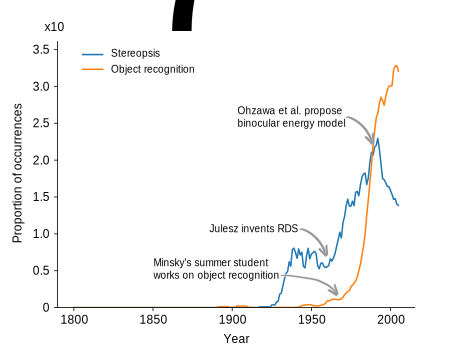
\includegraphics[keepaspectratio,width=9cm]{ngrams.pdf}
  \caption[Popularity of the n-grams `stereopsis' and `object recognition'.]{Popularity of the n-grams `stereopsis' and `object recognition'.}
  \label{fig:ch6fig1}
\end{figure}

To a non expert, figure \ref{fig:ch6fig1} might suggest that stereopsis is already well understood or that it is no longer an interesting research topic. In what follows I will argue that this is not the case. We still have a poor understanding of how different brain regions are involved stereoscopic vision. Beyond primary visual cortex, the scientific community has not yet managed to converge to a general computational framework for stereopsis, let alone designing mechanistic models that are able to predict neural responses to naturalistic 3D stimuli. Characterizing the contributions of different cortical layers is one promising line of research for exploring the interactions between different visual areas involved in stereopsis. In particular, it would be interesting to exploit the exploratory power of high-resolution functional magnetic resonance imaging to identify key circuits, which could then be dissected in greater detail using layer-specific electrical or optical recordings. The interactions between vergence, accommodation and stereopsis at the neural level are also poorly understood. There is evidence that disparity selectivity in V1 is greatly modulated by viewing distance \cite{Trotter:1992ij}, but, to my knowledge, models of disparity selectivity in V1 have yet to explain these findings.

Additionally, down-weighting the importance that studying stereopsis can have in advancing our understanding of the brain is a mistake. First, as I have mentioned before, stereopsis seems to rely on multiple brain regions across the entire brain, which attests its suitability to study how different brain regions work together to support perception. Second, stereopsis is a classical demonstration of how the brain excels at rapidly doing inverse graphics. Understanding how the brain achieves this may provide valuable insights to the fields of machine learning and artificial intelligence --- in the same way the connectionist principles inspired the development of modern, state-of-the-art artificial intelligence.


%%% ----------------------------------------------------------------------

% ------------------------------------------------------------------------

%%% Local Variables: 
%%% mode: latex
%%% TeX-master: "../thesis"
%%% End: 

% \include{conclusions/conclusions}

\backmatter % book mode only
% \appendix
% \include{appendix1/appendix1}
% \include{appendix2/appendix2}

\bibliographystyle{unsrtInitials}
%\bibliographystyle{Classes/CUEDbiblio}
%\bibliographystyle{Classes/jmb}
%\bibliographystyle{Classes/jmb} % bibliography style
\renewcommand{\bibname}{References} % changes default name Bibliography to References
\bibliography{/Users/nuno/Dropbox/NRG/library/ResearchLibrary_BibDesk}
% \bibliography{/Users/nuno/Sync/paper/ResearchLibrary_BibDesk.bib}

% \Bibliography{references/references} % References file

\end{document}
